
%% bare_jrnl.tex
%% V1.4b
%% 2015/08/26
%% by Michael Shell
%% see http://www.michaelshell.org/
%% for current contact information.
%%
%% This is a skeleton file demonstrating the use of IEEEtran.cls
%% (requires IEEEtran.cls version 1.8b or later) with an IEEE
%% journal paper.
%%
%% Support sites:
%% http://www.michaelshell.org/tex/ieeetran/
%% http://www.ctan.org/pkg/ieeetran
%% and
%% http://www.ieee.org/

%%*************************************************************************
%% Legal Notice:
%% This code is offered as-is without any warranty either expressed or
%% implied; without even the implied warranty of MERCHANTABILITY or
%% FITNESS FOR A PARTICULAR PURPOSE! 
%% User assumes all risk.
%% In no event shall the IEEE or any contributor to this code be liable for
%% any damages or losses, including, but not limited to, incidental,
%% consequential, or any other damages, resulting from the use or misuse
%% of any information contained here.
%%
%% All comments are the opinions of their respective authors and are not
%% necessarily endorsed by the IEEE.
%%
%% This work is distributed under the LaTeX Project Public License (LPPL)
%% ( http://www.latex-project.org/ ) version 1.3, and may be freely used,
%% distributed and modified. A copy of the LPPL, version 1.3, is included
%% in the base LaTeX documentation of all distributions of LaTeX released
%% 2003/12/01 or later.
%% Retain all contribution notices and credits.
%% ** Modified files should be clearly indicated as such, including  **
%% ** renaming them and changing author support contact information. **
%%*************************************************************************


% *** Authors should verify (and, if needed, correct) their LaTeX system  ***
% *** with the testflow diagnostic prior to trusting their LaTeX platform ***
% *** with production work. The IEEE's font choices and paper sizes can   ***
% *** trigger bugs that do not appear when using other class files.       ***                          ***
% The testflow support page is at:
% http://www.michaelshell.org/tex/testflow/



\documentclass[10pt,journal]{article}
%
% If IEEEtran.cls has not been installed into the LaTeX system files,
% manually specify the path to it like:
% \documentclass[journal]{../sty/IEEEtran}


% Some very useful LaTeX packages include:
% (uncomment the ones you want to load)


% *** MISC UTILITY PACKAGES ***
%
%\usepackage{ifpdf}
% Heiko Oberdiek's ifpdf.sty is very useful if you need conditional
% compilation based on whether the output is pdf or dvi.
% usage:
% \ifpdf
%   % pdf code
% \else
%   % dvi code
% \fi
% The latest version of ifpdf.sty can be obtained from:
% http://www.ctan.org/pkg/ifpdf
% Also, note that IEEEtran.cls V1.7 and later provides a builtin
% \ifCLASSINFOpdf conditional that works the same way.
% When switching from latex to pdflatex and vice-versa, the compiler may
% have to be run twice to clear warning/error messages.






% *** CITATION PACKAGES ***
%
\usepackage{cite}
% cite.sty was written by Donald Arseneau
% V1.6 and later of IEEEtran pre-defines the format of the cite.sty package
% \cite{} output to follow that of the IEEE. Loading the cite package will
% result in citation numbers being automatically sorted and properly
% "compressed/ranged". e.g., [1], [9], [2], [7], [5], [6] without using
% cite.sty will become [1], [2], [5]--[7], [9] using cite.sty. cite.sty's
% \cite will automatically add leading space, if needed. Use cite.sty's
% noadjust option (cite.sty V3.8 and later) if you want to turn this off
% such as if a citation ever needs to be enclosed in parenthesis.
% cite.sty is already installed on most LaTeX systems. Be sure and use
% version 5.0 (2009-03-20) and later if using hyperref.sty.
% The latest version can be obtained at:
% http://www.ctan.org/pkg/cite
% The documentation is contained in the cite.sty file itself.


%\usepackage[margin=1.5in]{geometry}
\usepackage{algorithm}
\usepackage{algpseudocode}
\makeatletter 
\renewcommand\thealgorithm{\thesection.\arabic{algorithm}} 
\@addtoreset{algorithm}{section} 
\makeatother
\usepackage{color,soul} %highlight 
% *** GRAPHICS RELATED PACKAGES ***
%
%\ifCLASSINFOpdf
  \usepackage[pdftex]{graphicx}
  % declare the path(s) where your graphic files are
  % \graphicspath{{../pdf/}{../jpeg/}}
  % and their extensions so you won't have to specify these with
  % every instance of \includegraphics
  % \DeclareGraphicsExtensions{.pdf,.jpeg,.png}
%\else
  % or other class option (dvipsone, dvipdf, if not using dvips). graphicx
  % will default to the driver specified in the system graphics.cfg if no
  % driver is specified.
  % \usepackage[dvips]{graphicx}
  % declare the path(s) where your graphic files are
  % \graphicspath{{../eps/}}
  % and their extensions so you won't have to specify these with
  % every instance of \includegraphics
  % \DeclareGraphicsExtensions{.eps}
%\fi
% % graphicx was written by David Carlisle and Sebastian Rahtz. It is
% % required if you want graphics, photos, etc. graphicx.sty is already
% % installed on most LaTeX systems. The latest version and documentation
% % can be obtained at: 
% % http://www.ctan.org/pkg/graphicx
% % Another good source of documentation is "Using Imported Graphics in
% % LaTeX2e" by Keith Reckdahl which can be found at:
% % http://www.ctan.org/pkg/epslatex
% %
% % latex, and pdflatex in dvi mode, support graphics in encapsulated
% % postscript (.eps) format. pdflatex in pdf mode supports graphics
% % in .pdf, .jpeg, .png and .mps (metapost) formats. Users should ensure
% % that all non-photo figures use a vector format (.eps, .pdf, .mps) and
% % not a bitmapped formats (.jpeg, .png). The IEEE frowns on bitmapped formats
% % which can result in "jaggedy"/blurry rendering of lines and letters as
% % well as large increases in file sizes.
% %
% % You can find documentation about the pdfTeX application at:
% % http://www.tug.org/applications/pdftex





% *** MATH PACKAGES ***
%
% \usepackage{amsmath}
\usepackage{amssymb}
\usepackage{mathtools} %includes and extends `amsmath'. Needed for dcases
% A popular package from the American Mathematical Society that provides
% many useful and powerful commands for dealing with mathematics.
%
% Note that the amsmath package sets \interdisplaylinepenalty to 10000
% thus preventing page breaks from occurring within multiline equations. Use:
\interdisplaylinepenalty=2500
% after loading amsmath to restore such page breaks as IEEEtran.cls normally
% does. amsmath.sty is already installed on most LaTeX systems. The latest
% version and documentation can be obtained at:
% http://www.ctan.org/pkg/amsmath

\usepackage{blkarray, bigstrut} %
\usepackage{kbordermatrix}% http://www.hss.caltech.edu/~kcb/TeX/kbordermatrix.sty
% *** SPECIALIZED LIST PACKAGES ***
%
\usepackage{algorithm}
\usepackage{algpseudocode}
% algorithmic.sty was written by Peter Williams and Rogerio Brito.
% This package provides an algorithmic environment fo describing algorithms.
% You can use the algorithmic environment in-text or within a figure
% environment to provide for a floating algorithm. Do NOT use the algorithm
% floating environment provided by algorithm.sty (by the same authors) or
% algorithm2e.sty (by Christophe Fiorio) as the IEEE does not use dedicated
% algorithm float types and packages that provide these will not provide
% correct IEEE style captions. The latest version and documentation of
% algorithmic.sty can be obtained at:
% http://www.ctan.org/pkg/algorithms
% Also of interest may be the (relatively newer and more customizable)
% algorithmicx.sty package by Szasz Janos:
% http://www.ctan.org/pkg/algorithmicx




% *** ALIGNMENT PACKAGES ***
%
\usepackage{array}
% Frank Mittelbach's and David Carlisle's array.sty patches and improves
% the standard LaTeX2e array and tabular environments to provide better
% appearance and additional user controls. As the default LaTeX2e table
% generation code is lacking to the point of almost being broken with
% respect to the quality of the end results, all users are strongly
% advised to use an enhanced (at the very least that provided by array.sty)
% set of table tools. array.sty is already installed on most systems. The
% latest version and documentation can be obtained at:
% http://www.ctan.org/pkg/array


% IEEEtran contains the IEEEeqnarray family of commands that can be used to
% generate multiline equations as well as matrices, tables, etc., of high
% quality.




% *** SUBFIGURE PACKAGES ***
%\ifCLASSOPTIONcompsoc
 \usepackage[caption=false,font=normalsize,labelfont=sf,textfont=sf,position=top]{subfig}
%\else
 %\usepackage[caption=false,font=footnotesize]{subfig}
%\fi
% subfig.sty, written by Steven Douglas Cochran, is the modern replacement
% for subfigure.sty, the latter of which is no longer maintained and is
% incompatible with some LaTeX packages including fixltx2e. However,
% subfig.sty requires and automatically loads Axel Sommerfeldt's caption.sty
% which will override IEEEtran.cls' handling of captions and this will result
% in non-IEEE style figure/table captions. To prevent this problem, be sure
% and invoke subfig.sty's "caption=false" package option (available since
% subfig.sty version 1.3, 2005/06/28) as this is will preserve IEEEtran.cls
% handling of captions.
% Note that the Computer Society format requires a larger sans serif font
% than the serif footnote size font used in traditional IEEE formatting
% and thus the need to invoke different subfig.sty package options depending
% on whether compsoc mode has been enabled.
%
% The latest version and documentation of subfig.sty can be obtained at:
% http://www.ctan.org/pkg/subfig




% *** FLOAT PACKAGES ***
%
% \usepackage{fixltx2e}
% fixltx2e, the successor to the earlier fix2col.sty, was written by
% Frank Mittelbach and David Carlisle. This package corrects a few problems
% in the LaTeX2e kernel, the most notable of which is that in current
% LaTeX2e releases, the ordering of single and double column floats is not
% guaranteed to be preserved. Thus, an unpatched LaTeX2e can allow a
% single column figure to be placed prior to an earlier double column
% figure.
% Be aware that LaTeX2e kernels dated 2015 and later have fixltx2e.sty's
% corrections already built into the system in which case a warning will
% be issued if an attempt is made to load fixltx2e.sty as it is no longer
% needed.
% The latest version and documentation can be found at:
% http://www.ctan.org/pkg/fixltx2e
\usepackage{epstopdf}

\usepackage{stfloats}
% stfloats.sty was written by Sigitas Tolusis. This package gives LaTeX2e
% the ability to do double column floats at the bottom of the page as well
% as the top. (e.g., "\begin{figure*}[!b]" is not normally possible in
% LaTeX2e). It also provides a command:
%\fnbelowfloat
% to enable the placement of footnotes below bottom floats (the standard
% LaTeX2e kernel puts them above bottom floats). This is an invasive package
% which rewrites many portions of the LaTeX2e float routines. It may not work
% with other packages that modify the LaTeX2e float routines. The latest
% version and documentation can be obtained at:
% http://www.ctan.org/pkg/stfloats
% Do not use the stfloats baselinefloat ability as the IEEE does not allow
% \baselineskip to stretch. Authors submitting work to the IEEE should note
% that the IEEE rarely uses double column equations and that authors should try
% to avoid such use. Do not be tempted to use the cuted.sty or midfloat.sty
% packages (also by Sigitas Tolusis) as the IEEE does not format its papers in
% such ways.
% Do not attempt to use stfloats with fixltx2e as they are incompatible.
% Instead, use Morten Hogholm'a dblfloatfix which combines the features
% of both fixltx2e and stfloats:
%
% \usepackage{dblfloatfix}
% The latest version can be found at:
% http://www.ctan.org/pkg/dblfloatfix




%\ifCLASSOPTIONcaptionsoff
%  \usepackage[nomarkers]{endfloat}
% \let\MYoriglatexcaption\caption
% \renewcommand{\caption}[2][\relax]{\MYoriglatexcaption[#2]{#2}}
%\fi
% endfloat.sty was written by James Darrell McCauley, Jeff Goldberg and 
% Axel Sommerfeldt. This package may be useful when used in conjunction with 
% IEEEtran.cls'  captionsoff option. Some IEEE journals/societies require that
% submissions have lists of figures/tables at the end of the paper and that
% figures/tables without any captions are placed on a page by themselves at
% the end of the document. If needed, the draftcls IEEEtran class option or
% \CLASSINPUTbaselinestretch interface can be used to increase the line
% spacing as well. Be sure and use the nomarkers option of endfloat to
% prevent endfloat from "marking" where the figures would have been placed
% in the text. The two hack lines of code above are a slight modification of
% that suggested by in the endfloat docs (section 8.4.1) to ensure that
% the full captions always appear in the list of figures/tables - even if
% the user used the short optional argument of \caption[]{}.
% IEEE papers do not typically make use of \caption[]'s optional argument,
% so this should not be an issue. A similar trick can be used to disable
% captions of packages such as subfig.sty that lack options to turn off
% the subcaptions:
% For subfig.sty:
% \let\MYorigsubfloat\subfloat
% \renewcommand{\subfloat}[2][\relax]{\MYorigsubfloat[]{#2}}
% However, the above trick will not work if both optional arguments of
% the \subfloat command are used. Furthermore, there needs to be a
% description of each subfigure *somewhere* and endfloat does not add
% subfigure captions to its list of figures. Thus, the best approach is to
% avoid the use of subfigure captions (many IEEE journals avoid them anyway)
% and instead reference/explain all the subfigures within the main caption.
% The latest version of endfloat.sty and its documentation can obtained at:
% http://www.ctan.org/pkg/endfloat
%
% The IEEEtran \ifCLASSOPTIONcaptionsoff conditional can also be used
% later in the document, say, to conditionally put the References on a 
% page by themselves.




% *** PDF, URL AND HYPERLINK PACKAGES ***
%
\usepackage{url}
% url.sty was written by Donald Arseneau. It provides better support for
% handling and breaking URLs. url.sty is already installed on most LaTeX
% systems. The latest version and documentation can be obtained at:
% http://www.ctan.org/pkg/url
% Basically, \url{my_url_here}.
\usepackage[hidelinks]{hyperref} % this should allow links (to sections but also to equations, figures, references) in pdf.



% *** Do not adjust lengths that control margins, column widths, etc. ***
% *** Do not use packages that alter fonts (such as pslatex).         ***
% There should be no need to do such things with IEEEtran.cls V1.6 and later.
% (Unless specifically asked to do so by the journal or conference you plan
% to submit to, of course. )


% Allow page breaks inside equations (or some other math environments). The optional argument ranges from 1 to 4. The higher the number, the more permissive you are of pagebreak
%\allowdisplaybreaks[1]

% An example of a floating figure using the graphicx package.
% Note that \label must occur AFTER (or within) \caption.
% For figures, \caption should occur after the \includegraphics.
% Note that IEEEtran v1.7 and later has special internal code that
% is designed to preserve the operation of \label within \caption
% even when the captionsoff option is in effect. However, because
% of issues like this, it may be the safest practice to put all your
% \label just after \caption rather than within \caption{}.
%
% Reminder: the "draftcls" or "draftclsnofoot", not "draft", class
% option should be used if it is desired that the figures are to be
% displayed while in draft mode.
%
%\begin{figure}[!t]
%\centering
%\includegraphics[width=2.5in]{myfigure}
% where an .eps filename suffix will be assumed under latex, 
% and a .pdf suffix will be assumed for pdflatex; or what has been declared
% via \DeclareGraphicsExtensions.
%\caption{Simulation results for the network.}
%\label{fig_sim}
%\end{figure}

% Note that the IEEE typically puts floats only at the top, even when this
% results in a large percentage of a column being occupied by floats.


% An example of a double column floating figure using two subfigures.
% (The subfig.sty package must be loaded for this to work.)
% The subfigure \label commands are set within each subfloat command,
% and the \label for the overall figure must come after \caption.
% \hfil is used as a separator to get equal spacing.
% Watch out that the combined width of all the subfigures on a 
% line do not exceed the text width or a line break will occur.
%
%\begin{figure*}[!t]
%\centering
%\subfloat[Case I]{\includegraphics[width=2.5in]{box}%
%\label{fig_first_case}}
%\hfil
%\subfloat[Case II]{\includegraphics[width=2.5in]{box}%
%\label{fig_second_case}}
%\caption{Simulation results for the network.}
%\label{fig_sim}
%\end{figure*}
%
% Note that often IEEE papers with subfigures do not employ subfigure
% captions (using the optional argument to \subfloat[]), but instead will
% reference/describe all of them (a), (b), etc., within the main caption.
% Be aware that for subfig.sty to generate the (a), (b), etc., subfigure
% labels, the optional argument to \subfloat must be present. If a
% subcaption is not desired, just leave its contents blank,
% e.g., \subfloat[].
%\usepackage{caption}
%\usepackage{subcaption}
\usepackage{tabularx}

% An example of a floating table. Note that, for IEEE style tables, the
% \caption command should come BEFORE the table and, given that table
% captions serve much like titles, are usually capitalized except for words
% such as a, an, and, as, at, but, by, for, in, nor, of, on, or, the, to
% and up, which are usually not capitalized unless they are the first or
% last word of the caption. Table text will default to \footnotesize as
% the IEEE normally uses this smaller font for tables.
% The \label must come after \caption as always.
%
%\begin{table}[!t]
%% increase table row spacing, adjust to taste
%\renewcommand{\arraystretch}{1.3}
% if using array.sty, it might be a good idea to tweak the value of
% \extrarowheight as needed to properly center the text within the cells
%\caption{An Example of a Table}
%\label{table_example}
%\centering
%% Some packages, such as MDW tools, offer better commands for making tables
%% than the plain LaTeX2e tabular which is used here.
%\begin{tabular}{|c||c|}
%\hline
%One & Two\\
%\hline
%Three & Four\\
%\hline
%\end{tabular}
%\end{table}


% Note that the IEEE does not put floats in the very first column
% - or typically anywhere on the first page for that matter. Also,
% in-text middle ("here") positioning is typically not used, but it
% is allowed and encouraged for Computer Society conferences (but
% not Computer Society journals). Most IEEE journals/conferences use
% top floats exclusively. 
% Note that, LaTeX2e, unlike IEEE journals/conferences, places
% footnotes above bottom floats. This can be corrected via the
% \fnbelowfloat command of the stfloats package.


% packages needed for plotting results
\usepackage{tikz}
\usetikzlibrary{trees}
\usepackage{pgfplots}
%\pgfplotsset{compat=1.15}
\usepackage{multirow}
\usepackage{booktabs} %for fancy tables
\usepackage{adjustbox}
\usepackage{multicol}
\usepackage{todonotes} 
% \usepackage[disable]{todonotes} %Hides all(!) todonotes
% todonotes appearance
\newcommand{\addref}{\todo[color=red!40,caption={}]{Add reference.}}
\newcommand{\rewrite}[1]{\todo[inline,color=yellow!40,caption={}]{#1}} % the caption={} is needed if you want to include itemize and such in the todonotes, see: https://tex.stackexchange.com/questions/54064/itemize-inside-todonote
\newcommand{\question}[1]{\todo[inline,color=blue!40,caption={}]{#1}}
\newcommand{\includes}[1]{\todo[inline,color=black!10,caption={}]{#1}}
% % Don't print any [non-inline] notes (will still show up in list of todo notes, to disable this, see: http://tex.stackexchange.com/questions/287394/todonotes-show-inline-hide-all-others)
% \makeatletter
% \renewcommand{\@todonotes@drawMarginNoteWithLine}{}
% \makeatother

\makeatletter
\renewcommand*\env@matrix[1][\arraystretch]{%
  \edef\arraystretch{#1}%
  \hskip -\arraycolsep
  \let\@ifnextchar\new@ifnextchar
  \array{*\c@MaxMatrixCols c}}
\makeatother

% Thick vertical line (") and thick horizontal line (\thickhline) for table
\makeatletter
\newcommand{\thickhline}{%
    \noalign {\ifnum 0=`}\fi \hrule height 1pt
    \futurelet \reserved@a \@xhline
}
\newcolumntype{"}{@{\hskip\tabcolsep\vrule width 1pt\hskip\tabcolsep}}
\makeatother

\usepackage[per-mode=symbol]{siunitx} %[per-mode=reciprocal]
% Define additional units
\DeclareSIUnit\radians{rad}
\DeclareSIUnit\perunit{p.u.}
\DeclareSIUnit\var{VAr}

% Define units with brackets around it
\makeatletter
\newcommand{\sib}[1]{$\left[\si{#1}\right]$}
\makeatother

\makeatletter
\newcommand{\SIB}[2]{$\left[\SI{#1}{#2}\right]$}
\makeatother

% Define appearance of vectors and matrices. Default for \vec{} is an arrow
% \renewcommand{\vec}[1]{\mathbf{#1}} %bold
\renewcommand{\vec}[1]{#1} %nothing
% \let\oldvec\vec
% \renewcommand{\vec}[1]{\oldvec{\mathbf{#1}}} %bold with arrow
% \newcommand{\matr}[1]{\mathbf{#1}} %bold
\newcommand{\matr}[1]{#1} %nothing

% Define appearence of imaginary unit
%\newcommand{\iu}{\tilde{i}\mkern1mu} %non-slanted i, with dot. This seems to be the `official' guideline (ISO standard?)
% \newcommand{\iu}{\iota} %iota (has no dot on the i)
\newcommand{\iu}{\imath} %has no dot on the i but is curly


% correct bad hyphenation here
\hyphenation{op-tical net-works semi-conduc-tor}


\begin{document}
%
% paper title
% Titles are generally capitalized except for words such as a, an, and, as,
% at, but, by, for, in, nor, of, on, or, the, to and up, which are usually
% not capitalized unless they are the first or last word of the title.
% Linebreaks \\ can be used within to get better formatting as desired.
% Do not put math or special symbols in the title.
\title{Solving the power flow problem on integrated transmission-distribution networks: a review and numerical assessment}
%
% author names and IEEE memberships
% note positions of commas and nonbreaking spaces ( ~ ) LaTeX will not break
% a structure at a ~ so this keeps an author's name from being broken across
% two lines.
% use \thanks{} to gain access to the first footnote area
% a separate \thanks must be used for each paragraph as LaTeX2e's \thanks
% was not built to handle multiple paragraphs
%

\author{~M.E.~Kootte,%~\IEEEmembership{Life~Fellow,~IEEE,}% <-this % stops a space
        ~J.E.~Romate,
        ~C.~Vuik%
% \thanks{M. Shell was with the Department
% of Electrical and Computer Engineering, Georgia Institute of Technology, Atlanta,
% GA, 30332 USA e-mail: (see http://www.michaelshell.org/contact.html).}% <-this % stops a space
% \thanks{J. Doe and J. Doe are with Anonymous University.}% <-this % stops a space
% \thanks{Manuscript received April 19, 2005; revised August 26, 2015.}%
}

% note the % following the last \IEEEmembership and also \thanks - 
% these prevent an unwanted space from occurring between the last author name
% and the end of the author line. i.e., if you had this:
% 
% \author{....lastname \thanks{...} \thanks{...} }
%                     ^------------^------------^----Do not want these spaces!
%
% a space would be appended to the last name and could cause every name on that
% line to be shifted left slightly. This is one of those "LaTeX things". For
% instance, "\textbf{A} \textbf{B}" will typeset as "A B" not "AB". To get
% "AB" then you have to do: "\textbf{A}\textbf{B}"
% \thanks is no different in this regard, so shield the last } of each \thanks
% that ends a line with a % and do not let a space in before the next \thanks.
% Spaces after \IEEEmembership other than the last one are OK (and needed) as
% you are supposed to have spaces between the names. For what it is worth,
% this is a minor point as most people would not even notice if the said evil
% space somehow managed to creep in.



% The paper headers
\markboth{Journal of \LaTeX\ Class Files,~Vol.~14, No.~8, August~2015}%
{Shell \MakeLowercase{\textit{et al.}}: Bare Demo of IEEEtran.cls for IEEE Journals}
% The only time the second header will appear is for the odd numbered pages
% after the title page when using the twoside option.
% 
% *** Note that you probably will NOT want to include the author's ***
% *** name in the headers of peer review papers.                   ***
% You can use \ifCLASSOPTIONpeerreview for conditional compilation here if
% you desire.




% If you want to put a publisher's ID mark on the page you can do it like
% this:
%\IEEEpubid{0000--0000/00\$00.00~\copyright~2015 IEEE}
% Remember, if you use this you must call \IEEEpubidadjcol in the second
% column for its text to clear the IEEEpubid mark.



% use for special paper notices
%\IEEEspecialpapernotice{(Invited Paper)}

% make the title area
\maketitle

% As a general rule, do not put math, special symbols or citations
% in the abstract or keywords.
\begin{abstract}
%Field, gap, fill, terugkoppeling 
\noindent Power flow simulations form an essential tool for electricity network analysis but conventional models are designed to work on a separated transmission or distribution network only. The continuing growth of electricity consumption, demand side participation and renewable resources makes the electricity networks co-dependent. Integrated models incorporate the coupling of the networks and interaction that they have on each other, representing the power flow within this changing environment accurately. \\ 
Several numerical methods are available to solve the power flow problem on integrated networks. They can be categorized as a unified or as a splitting method and networks can be modeled as a homogeneous or hybrid network. In this paper, we review and assess these methods on the network models by running simulations on small test networks and comparing the outcome on accuracy, computational time, and convergence. The review shows that all the methods solve the power flow problem accurately. Methods running on hybrid networks have a slight advantage in computational time. Realistic network models, running on millions of buses and with large distribution networks, should give a better insight into the speed of the computations. 
\end{abstract}

% Note that keywords are not normally used for peerreview papers.
%\begin{IEEEkeywords}
%nonlinear power flow, transmission-distribution, integrated networks, Newton-Raphson, convergence 
%\end{IEEEkeywords}


% For peer review papers, you can put extra information on the cover
% page as needed:
% \ifCLASSOPTIONpeerreview
% \begin{center} \bfseries EDICS Category: 3-BBND \end{center}
% \fi
%
% For peerreview papers, this IEEEtran command inserts a page break and
% creates the second title. It will be ignored for other modes.
%\IEEEpeerreviewmaketitle
\maketitle 

%-------------
% Introduction
%-------------
\section{Introduction}
%Field, Gap, Focus 
Power flow computations are used to simulate the transport, generation, and consumption of power in electricity networks. The simulations are important for safe operation and planning of the electricity grid \todo{source}. A national electricity grid consists of one transmission network, responsible for transport of power over large distances, and several distribution networks, responsible for the transport to end-consumers. Transmission networks transport high-voltage power to substations from where power is converted to a lower voltage level. The distribution network transports low-voltage power from substations to end-consumers. These transmission and distribution domains are currently separately analyzed: In the analysis of the first, the transmission network is modeled in detail while the distribution network is modeled as an equivalent load. In the analysis of the distribution system, this system is modeled in detail while the transmission network is simplified as a power supply source.  \newline\newline
The power system is changing: 1) more renewable energy is entering the grid at distribution level, 2) we see an increase of demand-side participation as a mechanism to balance frequency, and 3) we see an increase of electricity consumption\todo{source}. The changing environment requires a more detailed analysis of the electricity network and a more complex model of the interaction between the networks. Integrated transmission-distribution network models study the interaction that these networks have on each other. But it is not straight-forward to integrate these separate domains. The networks have different characteristics what has resulted in different network models that cannot be easily integrated. The most important difference is that the transmission network is a balanced network: Power is generated in three phases but voltage and current of other phases have the same magnitude and are equally shifted in phase by $2/3\pi$ rad. Therefore, the transmission network is modeled in single-phase while the distribution network is in general not balanced and thus modeled in three-phase \todo{source}. 
Furthermore, the different characteristics have lead to the development of different algorithms to solve the power flow problem of different systems. The power flow problem is a nonlinear problem which is solved using iterative methods. Well-known algorithms to solve transmission systems are: Gauss-Seidel, Newton-Raphson, Decoupled loadflow, and DC loadflow \cite{Schavemaker2008chap6}. These solvers have been adapted to distribution solvers, among which the most well-known are: Newton-Raphson current mismatch \cite{Garcia2000}\cite{Abdel-akher2005}, implicit $Z_{bus}$ \cite{Teng2002a}\cite{Chen1991a}, BIBC/BCBV \cite{Teng2008}\cite{Farag2011}, and Forward/Backward Sweep \cite{Moghaddas2009}\cite{Eminoglu2008} methods. Besides the technical complexity of integrating network models, we have the issue of confidentiality. System operators, the instances responsible for safe operation of their electricity grid,  are not willing or not allowed to share network information with other system operators\todo{source}. One can reason that the ongoing energy transition and electrification is going to push the limits of conventional models until they do not suffice anymore.  It is probable that legislation and current behaviour will then follow the necessary change towards the use of integrated network models. 
\newline\newline 
The study of integrated network models is an emerging field. A literature review shows that multiple approaches exist that can roughly be categorized into 1) co-simulation frameworks that combine multiple domains that can be studied using different \textit{formats} and 2) stand-alone analysis frameworks that study integrated network models using the same \textit{software tools} \cite{https://ieeexplore.ieee.org/stamp/stamp.jsp?tp=&arnumber=8585926}. Co-simulation frameworks are modular and well-suited for HPC architectures which make them ideal for simultaneous analysis of large transmission and distribution networks (100s to 1000s of buses) \cite{https://www.nrel.gov/docs/fy16osti/65550.pdf}. Stand-alone frameworks have been depreciated by the co-simulation community because of the high costs of simulation \cite{https://ieeexplore.ieee.org/stamp/stamp.jsp?tp=&arnumber=8585926}. While efficiently integrated stand-alone models require significantly less communication and should therefore be compatible with co-simulation techniques. Literature shows that studies focusing on stand-alone models have \textit{thus far} resulted in the creation of different modeling techniques. These techniques have been tested on small-size transmission and distribution networks in order to check their feasibility \cite{Taranto2008}\cite{Sun2015}. In this work, we give an insight in the performance of the stand-alone methods and their ability to be efficiently scaled to large-size networks: We compare the existing stand-alone methods on convergence and CPU-time by applying them on several transmission-distribution networks. The contributions of this work can be summarized as follows: 
\begin{itemize}
    \item An extensive description of existing stand-alone methods that have been categorized according their modeling and integration approach. Network models can be divided into hybrid and homogeneous network models. A homogeneous network model is a three-phase representation of both the transmission and distribution network. A hybrid network model consists of a single-phase transmission and a three-phase distribution network. Stand-alone integration approaches can be classified as a unified \cite{Taranto2008} or as a splitting method \cite{Sun2005}. The unified method  solves the integrated system as a whole. The splitting method is similar to the co-simulation approach where the separate domains are solved on its own and coupled using an iterative approach;
    \item A comparison of these methods using Matlab \todo{source} in which several test-cases are created to simulate the convergence behavior, where special attention is paid to CPU-time and number of iterations;
    \item An analysis of convergence characteristics under varying circumstances such as a high level of distributed generation and the integration of multiple distribution networks into one transmission-network;
    \item An insight into how these methods should adapt according to HPC applications in order to solve realistically sized networks (up to 1000000s buses). 
\end{itemize}


% Integrated networks can be modeled as homogeneous and as hybrid networks. A homogeneous network model is a three-phase representation of both the transmission and distribution network. A hybrid network model consists of a single-phase transmission and a three-phase distribution network. Several numerical methods have been developed to solve integrated networks. They can be classified as a unified \cite{Taranto2008} or as a splitting method \cite{Sun2005}.  The unified methods solve the integrated system as a whole. The splitting method divides the networks into a manager and a fellow and defines an extra iterative scheme between them. At every iteration, the separated systems are solved on its own. The integrated system is solved once convergence on the boundary between the systems have been reached. This article reviews the proposed integration methods and analyzes them by running simulations on small test-cases. We pay special attention to their convergence behaviour: CPU-time and the number of iterations. 


\section{Characterization of the power flow problem}
The steady-state power flow problem is the problem of determining the voltages $V$ in a network, given the specified power\footnote{We use the subscript $\iota$ as the imaginary unit.} $S=P+\iota Q$ and current $I$. $V$ and $I$ are related by Ohm's Law, $I = YV$, and $S$ and $V$ are related by $S=VI^*$. $Y$ represents the admittance of a power cable. Power is generated in three phases leading to three sinusoidal functions that describe phase $a$, $b$, and $c$ of the voltage and of the current. The voltage and current are both expressed in phasor notation: 
   \begin{align}
    V_p &=|V|_p\exp{(\iota\delta_{V_p}-\phi_{p})},\\
    I_p &=|I|_p\exp{(\iota\delta_{I_p}-\phi_{p})},\quad\ p\in\{a,b,c\},
    \end{align}
where $|\cdot|$ describes the phasor magnitude, $\delta_*$ the phase angle, and $\phi_*$ the phase shift. Phasors are often expressed as $V=\{|V|,\delta\}$. 
Current is never specified in an electricity system, therefore we substitute Ohm's Law into $S=VI^*$ and get a nonlinear equation for $S$, the three-phase nonlinear power flow equation, described as follows:  
\begin{align}
    S_p=V_p(\mathbf{Y}V)_p^*,\quad\ p\in\{a,b,c\}.
    \label{eq:SVYVp}
\end{align}
We represent an electricity network as a graph consisting of buses $i=1,..,N$ and branches (named after the two surrounding buses). These buses are either a load bus (PQ bus), a generator bus (PV bus), or a reference bus, depending on the information we know at that point. The loads in a network are modeled as PQ buses, loads consume power and at this bus, the active (P) and reactive power (Q) are specified.  Generators are modeled as PV buses, except for the first generator in a network, this bus is modeled as the slack bus. Generators supply power and at this bus, the active power (P) and voltage magnitude ($|V|$) are specified. At a slack bus, the voltage magnitude and angle are specified. This is summarized in table \ref{tab:networknodes}. 
\begin{table}[htbp]
\centering
\caption{Bustypes in a network and the information we know and not know at each bus $i$. }
\label{tab:networknodes}
\begin{tabular}{llllll}
\toprule
bus type  &&& \multicolumn{1}{c}{known} && \multicolumn{1}{c}{unknown} \\ \hline
$PQ$-bus  &&& $P_i,\ Q_i$               && $\delta_i,\ |V_i|$          \\
$PV$-bus  &&& $P_i,\ |V_i|$             && $Q_i,\ \delta_i$            \\
slack bus &&& $\delta_i,\ |V_i|$        && $P_i,\ Q_i$          \\      
\toprule
\end{tabular}
\end{table}
We scale all the engineering quantities in the power system to per-unit (pu) quantities by dividing them by their base value. In this way, we bring the voltage in a narrow range close to unity to eliminate erroneous values \cite{Schavemaker2008chap6}. \newline
Equation \eqref{eq:SVYVp} is a nonlinear equation so we solve it using iterative methods. At each node $i$, we solve the following equation for the unknown quantities:
\begin{align}
       S_i=V_i\sum_{k=1}^N{\mathbf{Y}}^*_{ik}{V}^*_k \label{eq:SVI}
\end{align}
The nodal admittance matrix $\mathbf{Y}_{ij}$ consists of admittance $y_{ij}$ of a line between node $i$ and $j$ and nodal shunt susceptance $b_c$. Line admittance consists of a real and imaginary part: $y_{ij}= 1/z_{ij}= 1 / (r_{ij}+\iota x_{ij})$, $z$ being impedance, $r$ being resistance and $x$ being reactance.  The nodal admittance matrix relating node $i$ and $j$ looks as the following: 
\begin{align}\mathbf{Y}_{ij}= 
\begin{bmatrix}
(y_{ij}+\iota \frac{b_c}{2})\frac{1}{\tau^2} & -y_{ij}\frac{1}{\tau\exp{(-\iota\theta_s)}}\nonumber \\
-y_{ij}\frac{1}{\tau\exp{(\iota\theta_s)}}& y_{ij}+\iota \frac{b_c}{2}   
\end{bmatrix} = \begin{bmatrix} Y_{11} & Y_{12} \\ Y_{21} & Y_{22}
\end{bmatrix}_{ij}
\end{align}
The parameters $\theta_s$ and $\tau$ are the transformer's phase-shift angle and tap ratio, when there is no transformer between two nodes but just a normal power cable, $\theta_s=0$ and $\tau=1$. 

\section{Electricity networks}
An electricity network consists of one transmission and several distribution networks. The design and characteristics of these types are different and therefore require different approaches to solve equation \eqref{eq:SVYVp}.
\subsection{Transmission networks: single-phase representation}
The transmission network is the high-voltage network, responsible for the transportation of power over large distances. It is a balanced system which means that the three phases $a,\ b,$ and $c$ of the generated power are equal in magnitude and equal in phase-shift ($\phi$). For a voltage $V$ this means that $|V|_a=|V|_b=|V|_c$ and $\phi_{ab}=\phi_{bc}=\phi_{ca}=\frac{2}{3}\pi$. 
To simplify and speed-up the computations in the transmission network, they only calculate $V_a$ and deduct the other two phases from here. This changes \eqref{eq:SVYVp} into the following: 
\begin{align}
    S_p=V_p(YV)_p^*,\quad\ p\in\{a,b,c\}\quad \Rightarrow \quad S_a=V_a(YV)_a^*
    \label{eq:SVYVa}.
\end{align}
We use Newton-Raphson power mismatch (NR-power) to compute unknown quantities at each bus $i$. NR-power computes $V_i$ using the following power mismatch formulation:
\begin{align}
    \Delta S_i = S_{s,i} - S(V_i) \approx 0.
\end{align}
$S_s$ is the specified power, the known information at generator and load nodes: $S_s=S_g-S_d$, subscript $g$ representing the generator buses and $d$ the load buses. $S(V)$ is the injected power, $S(V)=V({\mathbf{Y}V})^*$. 
The complex power $S$ is split into an active and reactive part and combined to form the power mismatch vector $F$, 
\begin{align}
     F(V)=\begin{bmatrix}
                \Delta {P}\\ \Delta {Q}
               \end{bmatrix}  = \begin{bmatrix}
               {P}_s-{P}(V) \\ {Q}_s-{Q}(V)
               \end{bmatrix}.
    \label{eq:powmism}
\end{align}
We denote the state variables $V$ by $x$, $x:=V=\{|V|,\delta\}$. We compute $V$ in an iterative manner using the Jacobian $J$ of the power mismatch vector: 
\begin{align}
  {\Delta x^\nu} &= \mathbf{-J^{-1}}(x^\nu )F(x^\nu),\\
  {x^{\nu +1}} &= {x^\nu + \Delta x^\nu}, 
  \end{align}  where the Jacobian is represented as follows: 
  $$\mathbf{J}({x})=\begin{bmatrix}
\frac{\partial P}{\partial\delta} & \frac{\partial P}{\partial|V|}  \\ 
\frac{\partial Q}{\partial\delta} & \frac{\partial Q}{\partial|V|} \end{bmatrix}.$$   
We repeat this until the norm of the power mismatch vector $|{F}|_{\infty}$ is lower than a certain tolerance value $\epsilon$. We choose $\epsilon=10^{-8}$ and start with a flat profile as initial guess: $V^0=0$.  
The Newton-Raphson algorithm is as follows: 
\begin{algorithm}
 \caption{The Newton-Raphson iterative method}
 \label{alg:NR}
 \begin{algorithmic}[1]
 \State Set $\nu=0$ and choose appropriate starting value $\mathbf{x}^0$;
 \State Compute ${F(x^\nu)}$;
 \State Test convergence: If $|{F}({x^\nu)}|_{\infty}\leq\epsilon$  then ${x}^\nu$ is the solution,
 Otherwise continue. 
 \State Compute the Jacobian matrix $\mathbf{J}(x^\nu)$;
 \State Update the solution: 
 \begin{equation*}
  \begin{aligned}
 {\Delta x^\nu} &= \mathbf{-J^{-1}}(x^\nu )F(x^\nu)\\
  {x^{\nu +1}} &= {x^\nu + \Delta x^\nu}
  \end{aligned}
 \end{equation*}
\State Update iteration counter $\nu+1\rightarrow \nu$, go to step 2.  
 \end{algorithmic}
\end{algorithm}{}


\subsection{Distribution networks: three-phase representation}
Distribution systems are unbalanced: the three phases are not equal in magnitude nor in phase-shift. This requires us to compute all the three phases in every iteration when solving equation \eqref{eq:SVYVp}. We use Newton-Raphson Three-Phase Current Injection Method (NR-TCIM) \cite{Garcia2000} to solve distribution networks. Instead of applying the standard Newton-Raphson method to power mismatches, Ohm's Law  is directly used resulting in the current mismatch vector: 
\begin{align}
     {F}({x})=\begin{bmatrix}
                \Delta {I}^{Re,abc}({x})\\ 
                \Delta {I}^{Im,abc}({x}) 
               \end{bmatrix}  = \begin{bmatrix}
   {I}_s^{Re,abc} - {I}^{Re,abc}({x}) \\
   {I}_s^{Im,abc} - {I}^{Im,abc}({x})
               \end{bmatrix}.
    \label{eq:curmism}
\end{align}
The specified current ${I_s}$ and computed current ${I}\left({V}\right)$ are calculated using the injected complex power and Ohm's Law: 
\begin{align}
    {I_{s,i}} = \left(\frac{\overline{S_s}}{V}\right)_i\quad\mbox{and}\quad I(V)_i = \mathbf{Y}V_i 
\end{align}
The Jacobian is formed by taking the derivative of the real and imaginary current mismatch with respect to the real and imaginary voltage.
\subsection{Modeling elements in three-phase configuration}
An electricity network models consists of nodal and series elements. Loads, generators, and shunts are nodal elements and are taken into account in the complex power vector $\mathbf{S}$. Transformers, line elements, and regulators are placed in series. They are accounted for in the $Y_{bus}$ matrix. Regulators are elements that are placed alone the distribution feeder to regulate the voltage profile of the feeder.  
\subsubsection{Loads and shunts}
Loads are modeled as buses where active and reactive power ($P$ and $Q$) are specified. They are modeled as a function of the voltage in which the load-model type determines the relation between power and voltage. Three types exist: the constant power (P), constant current (I), and constant impedance model (Z). Together called: ZIP-load models.    
\begin{enumerate}
    \item Constant Power models (P): power is independent of the change in voltage magnitude, which is expressed as: $$
    \frac{P}{P_0} =1 \quad\mbox{and}\quad \frac{Q}{Q_0}=1
    $$
    Constant power loads draw the same power from its source even if the source changes voltage.
    \item Constant Current models (I): power is related to the voltage magnitude as: $$
        \frac{P}{P_0} =\frac{|V|}{|V_0|} \quad\mbox{and}\quad \frac{Q}{Q_0}=\frac{|V|}{|V_0|}
    $$
    A constant current load varies its internal resistance according to the voltage which is being fed to it in order to achieve a constant current despite fluctuations in the source voltage.  
    % \hl{quote: A constant current load is one which varies its internal resistance to achieve a constant current regardless of the voltage which is being fed to it and therefore the power will vary. In other words, a constant current load would draw approx the same amount of current, despite wide variations in the source voltage or other impedances in the circuit.}
    \item Constant Impedance models (Z): power is related to the square of the voltage magnitude: $$
        \frac{P}{P_0} =(\frac{|V|}{|V_0|})^2 \quad\mbox{and}\quad \frac{Q}{Q_0}=(\frac{|V|}{|V_0|})^2
    $$
    A constant impedance load presents the same impedance even when voltage is fluctuating. 
\end{enumerate}
\hl{The $|V_0|$ is the nominal voltage magnitude. In p.u. calculations, this is equal to 1. }\\ 
Loads are physically connected in a grounded Wye or ungrounded Delta configuration. In the grounded Wye configuration all the three phases are connected to a single neutral point. This neutral point is connected to the ground by a fourth wire: the neutral conductor. The voltage is specified line-to-neutral.
In an ungrounded Delta configuration the loads are connected phase-to-phase without a neutral conductor. Here, the voltage is specified phase-to-phase, also called line-to-line. The line-to-line voltages of a three-phase Delta-configuration are: $V^{ab}$, $V^{bc}$, and $V^{ca}$.  The line-to-line voltages and line-to-neutral voltages ($V^a$, $V^b$, and $V^c$) are related as follows:
\begin{align}
    V^{ab} = V^a - V^b,\\ 
    V^{bc} = V^b - V^c,\\ 
    V^{ca} = V^c - V^a.\\ 
\end{align}
The line-to-neutral currents are related to line-to-line voltages according: 
\begin{align}
    I^a=I^{ab}-I^{ca},\\
    I^b=I^{bc}-I^{ab},\\
    I^c=I^{ca}-I^{bc}.
\end{align}
In the following lines we clarify the relationship of the ZIP-load models in a Wye and Delta configuration. 
\subparagraph{Wye - P}
We know that power is independent of voltage magnitude: \begin{equation}
    \frac{P}{P_0}=1,\ \frac{Q}{Q_0}=1\ \Leftrightarrow\ S := P +\iota Q = P_0 + \iota Q_0
\end{equation}
For phases $a$, $b$, and $c$ this means that for each load bus $i$ the active and reactive power are expressed as follows: 
\begin{align}
    \begin{bmatrix}
    S^a\\
    S^b\\
    S^c
    \end{bmatrix}_i := \begin{bmatrix}
    P^a +\iota Q^a\\
    P^b +\iota Q^b\\
    P^c +\iota Q^c
    \end{bmatrix}_i = \begin{bmatrix}
    P^a_0 +\iota Q^a_0\\
    P^b_0 +\iota Q^b_0\\
    P^c_0 +\iota Q^c_0
    \end{bmatrix}_i 
\end{align}
\subparagraph{Wye - I}
Constant current load models vary their power $S$ with voltage magnitude, leading to the following relationship: 
\begin{equation}
    \frac{P}{P_0}=|V|,\ \frac{Q}{Q_0}=|V|\ \Leftrightarrow\ S := P +\iota Q = (P_0 + \iota Q_0)|V|
\end{equation}
For phases $a$, $b$, and $c$ this means that for each load bus $i$ the active and reactive power are expressed as follows: 
\begin{align}
    \begin{bmatrix}
    S^a\\
    S^b\\
    S^c
    \end{bmatrix}_i := \begin{bmatrix}
    P^a +\iota Q^a\\
    P^b +\iota Q^b\\
    P^c +\iota Q^c
    \end{bmatrix}_i = \begin{bmatrix}
    (P^a_0 +\iota Q^a_0)(|V^a|)\\
    (P^b_0 +\iota Q^b_0)(|V^b|)\\
    (P^c_0 +\iota Q^c_0)(|V^c|)
    \end{bmatrix}_i 
\end{align}
\subparagraph{Wye - Z}
Constant impedance models vary their power with the square of voltage magnitude, leading to the following: 
\begin{equation}
    \frac{P}{P_0}=|V|^2,\ \frac{Q}{Q_0}=|V|^2\ \Leftrightarrow\ S := P +\iota Q = (P_0 + \iota Q_0)|V|^2
\end{equation}
For phases $a$, $b$, and $c$ this means that for each load bus $i$ the active and reactive power are expressed as follows: 
\begin{align}
    \begin{bmatrix}
    S^a\\
    S^b\\
    S^c
    \end{bmatrix}_i := \begin{bmatrix}
    P^a +\iota Q^a\\
    P^b +\iota Q^b\\
    P^c +\iota Q^c
    \end{bmatrix}_i = \begin{bmatrix}
    (P^a_0 +\iota Q^a_0)(|V^a|^2)\\
    (P^b_0 +\iota Q^b_0)(|V^b|^2)\\
    (P^c_0 +\iota Q^c_0)(|V^c|^2)
    \end{bmatrix}_i 
\end{align}
We solve the three-phase distribution systems with the NR-TCIM method, which implies that we need the specified currents $I_s$ in our mismatch equation (eq: \ref{eq:curmism}) instead of specified powers. As currents are never measured in a power system, they are conducted from the specified power according the relationship: 
\begin{equation}
    S=VI^*\ \Leftrightarrow\ I = (\frac{S}{V})^*
\end{equation}
If we divide the expressions of the loads $S$ by $V$ and take the conjugate of this new relation we get the load models expressions in terms of specified current:
\subparagraph{Wye - P }
\begin{equation}
    I := (\frac{S}{V})^* = (\frac{P_0+\iota Q_0}{V})^*
\end{equation}
Or in three-phase matrix: 
\begin{align}
\begin{bmatrix}
    I^a\\
    I^b\\
    I^c
    \end{bmatrix}_i = \begin{bmatrix}
   (\frac{ P^a +\iota Q^a}{V^a})^*\\
    (\frac{ P^b +\iota Q^b}{V^b})^*\\
    (\frac{ P^c +\iota Q^c}{V^c})^*
    \end{bmatrix}_i 
    \end{align}
\subparagraph{Wye - I }
\begin{equation}
    I := (\frac{S|V|}{V})^* = (P_0+\iota Q_0)^*\frac{|V|}{V^*} = (P_0+\iota Q_0)^*\frac{V}{|V|}
\end{equation}
Or in three-phase matrix: 
\begin{align}
\begin{bmatrix}
    I^a\\
    I^b\\
    I^c
    \end{bmatrix}_i = \begin{bmatrix}
    ({ P^a +\iota Q^a})^*\frac{V^a}{|V^a|}\\
    ({ P^b +\iota Q^b})\frac{V^b}{|V^b|}\\
    ({ P^c +\iota Q^c})^*\frac{V^c}{|V^c|})
    \end{bmatrix}_i 
    \end{align}
    
\subparagraph{Wye - Z }
\begin{equation}
    I := (\frac{S|V|^2}{V})^* = ({P_0+\iota Q_0})^*\frac{|V|^2}{V^*} = ({P_0+\iota Q_0})^*\frac{VV^*}{V^*} =  ({P_0+\iota Q_0})^*V
\end{equation}
Or in three-phase matrix: 
\begin{align}
\begin{bmatrix}
    I^a\\
    I^b\\
    I^c
    \end{bmatrix}_i = \begin{bmatrix}
   ({ P^a +\iota Q^a})^*{V^a}\\
    ({ P^b +\iota Q^b})^*{V^b}\\
    ({ P^c +\iota Q^c})^*{V^c}
    \end{bmatrix}_i 
    \end{align}
\paragraph{Delta loads}
Delta loads are expressed by line-to-line voltages and currents while we need line-to-neutral currents in our calculations. We express the line-to-neutral currents directly for the three load models using \begin{align}
    I^a=I^{ab}-I^{ca},\\
    I^b=I^{bc}-I^{ab},\\
    I^c=I^{ca}-I^{bc}.
\end{align}
\subparagraph{Delta - P}
\begin{align}
\begin{bmatrix}
    I^a\\
    I^b\\
    I^c
    \end{bmatrix}_i := \begin{bmatrix}
    I^{ab}-I^{ca}\\
    I^{bc}-I^{ab}\\
    I^{ca}-I^{bc}
    \end{bmatrix}_i = \begin{bmatrix}
   (\frac{ P^{ab} +\iota Q^{ab}}{V^a-V^b})^* - (\frac{ P^{ca} +\iota Q^{ca}}{V^c-V^a})^* \\
    (\frac{ P^{bc} +\iota Q^{bc}}{V^b-V^c})^* - (\frac{ P^{ab} +\iota Q^{ab}}{V^a-V^b})^*\\
    (\frac{ P^{ca} +\iota Q^{ca}}{V^c-V^a})^* - (\frac{ P^{bc} +\iota Q^{bc}}{V^b-V^c})^*
    \end{bmatrix}_i 
    \end{align}
\subparagraph{Delta - I }
\begin{align}
\begin{bmatrix}
    I^a\\
    I^b\\
    I^c
    \end{bmatrix}_i = \begin{bmatrix}
    ({ P^{ab} +\iota Q^{ab}})^*\frac{(V^a-V^b)}{|V^a-V^b|} - ({ P^{ca} +\iota Q^{ca}})^*\frac{(V^c-V^a)}{|V^c-V^a|}  \\
    ({ P^{bc} +\iota Q^{bc}})^*\frac{(V^b-V^c)}{|V^b-V^c|} - ({ P^{ab} +\iota Q^{ab}})^*\frac{(V^a-V^b)}{|V^a-V^b|}\\
    ({ P^{ca} +\iota Q^{ca}})^*\frac{(V^c-V^a)}{|V^c-V^a|} -  ({ P^{bc} +\iota Q^{bc}})^*\frac{(V^b-V^c)}{|V^b-V^c|}
    \end{bmatrix}_i 
    \end{align}
    
\subparagraph{Delta - Z }
 
\begin{align}
\begin{bmatrix}
    I^a\\
    I^b\\
    I^c
    \end{bmatrix}_i = \begin{bmatrix}
   ({ P^{ab} +\iota Q^{ab}})^*{(V^a-V^b)} - ({ P^{ca} +\iota Q^{ca}})^*{(V^c-V^a)} \\
     ({ P^{bc} +\iota Q^{bc}})^*{(V^b-V^c)} -  ({ P^{ab} +\iota Q^{ab}})^*{(V^a-V^b)}\\
    ({ P^{ca} +\iota Q^{ca}})^*{(V^c-V^a)} - ({ P^{bc} +\iota Q^{bc}})^*{(V^b-V^c)}
    \end{bmatrix}_i 
    \end{align}

\paragraph{Overview of load models}
 We give an overview of the three constant load models (P, I, and Z) in Wye and Delta configuration.
 \begin{table}[h]
\renewcommand{\arraystretch}{1.3}
\centering
\caption{Specified line-to-neutral currents of load bus $i$ in Wye and Delta configuration, given for different load models (ZIP). }\label{tab:ZIPmodels}
\begin{adjustbox}{width=1\textwidth} %, angle=90}
\small
\begin{tabular}{ccccc}
\toprule
{} && {Y} && {$\Delta$}  \\

 load model &&        Wye  &&        Delta\\
\midrule
Z   &&  $  \begin{bmatrix}
   ({ P^a +\iota Q^a})^*{V^a}\\
    ({ P^b +\iota Q^b})^*{V^b}\\
    ({ P^c +\iota Q^c})^*{V^c}
    \end{bmatrix}_i $ && $  \begin{bmatrix}
   ({ P^{ab} +\iota Q^{ab}})^*{(V^a-V^b)} - ({ P^{ca} +\iota Q^{ca}})^*{(V^c-V^a)} \\
     ({ P^{bc} +\iota Q^{bc}})^*{(V^b-V^c)} -  ({ P^{ab} +\iota Q^{ab}})^*{(V^a-V^b)}\\
    ({ P^{ca} +\iota Q^{ca}})^*{(V^c-V^a)} - ({ P^{bc} +\iota Q^{bc}})^*{(V^b-V^c)}
    \end{bmatrix}_i $  \\  \midrule 
I   &&  $ \begin{bmatrix}
    ({ P^a +\iota Q^a})^*\frac{V^a}{|V^a|}\\
    ({ P^b +\iota Q^b})\frac{V^b}{|V^b|}\\
    ({ P^c +\iota Q^c})^*\frac{V^c}{|V^c|})
    \end{bmatrix}_i  $ &&   $ \begin{bmatrix}
    ({ P^{ab} +\iota Q^{ab}})^*\frac{(V^a-V^b)}{|V^a-V^b|} - ({ P^{ca} +\iota Q^{ca}})^*\frac{(V^c-V^a)}{|V^c-V^a|}  \\
    ({ P^{bc} +\iota Q^{bc}})^*\frac{(V^b-V^c)}{|V^b-V^c|} - ({ P^{ab} +\iota Q^{ab}})^*\frac{(V^a-V^b)}{|V^a-V^b|}\\
    ({ P^{ca} +\iota Q^{ca}})^*\frac{(V^c-V^a)}{|V^c-V^a|} -  ({ P^{bc} +\iota Q^{bc}})^*\frac{(V^b-V^c)}{|V^b-V^c|}
    \end{bmatrix}_i $  \\ \midrule 
P   &&  $ \begin{bmatrix} 
   (\frac{ P^a +\iota Q^a}{V^a})^*\\
    (\frac{ P^b +\iota Q^b}{V^b})^*\\
    (\frac{ P^c +\iota Q^c}{V^c})^*
    \end{bmatrix}_i $ &&   $  \begin{bmatrix}
   (\frac{ P^{ab} +\iota Q^{ab}}{V^a-V^b})^* - (\frac{ P^{ca} +\iota Q^{ca}}{V^c-V^a})^* \\
    (\frac{ P^{bc} +\iota Q^{bc}}{V^b-V^c})^* - (\frac{ P^{ab} +\iota Q^{ab}}{V^a-V^b})^*\\
    (\frac{ P^{ca} +\iota Q^{ca}}{V^c-V^a})^* - (\frac{ P^{bc} +\iota Q^{bc}}{V^b-V^c})^*
    \end{bmatrix}_i $ \\

\bottomrule
\end{tabular}
\end{adjustbox}
\end{table}


\subsubsection{Transformers}
Transformers are placed between two networks that have different voltage levels. The primary side ($p$) of the transformer is connected to the higher voltage network and the secondary side ($s$) is connected to the lower voltage level. The transformer in a power system is represented by two blocks:
\begin{itemize}
    \item An admittance matrix block, $Y^{abc}_T$, consisting of per-unit leakage admittance $y_t$, and  
    \item A shunt block that models core losses. The shunt block can be represented by voltage dependent loads and follow the representation in Tab. \ref{tab:ZIPmodels}. 
\end{itemize}
The admittance matrix block is given in a similar manner as the $Y_{bus}$ matrix of a distribution cable, but now consisting of leakage admittance of the transformer: \begin{equation}
    Y^{abc}_T = \begin{bmatrix}
    Y_{pp}^{abc} & Y^{abc}_{ps} \\
     Y_{sp}^{abc} & Y^{abc}_{ss}
    \end{bmatrix}.
\end{equation}
Each block $Y^{abc}_{ij}$, $i,j\in\{p,s\}$ has a different configuration. This configuration depends on the connection of the transformer and is either one of the three following blocks: \begin{equation}\resizebox{0.91\columnwidth}{!}{%
$
    Y_1=\begin{bmatrix}
    y_t & 0 & 0 \\
    0 & y_t & 0 \\
    0 & 0 & y_t
    \end{bmatrix},\quad Y_2=\frac{1}{3}\begin{bmatrix}
    2y_t & -y_t & -y_t \\
    -y_t & 2y_t & -y_t \\
    -y_t & -y_t & 2y_t
    \end{bmatrix},\quad\mbox{and}\quad Y_3=\frac{1}{\sqrt{3}}\begin{bmatrix}
    -y_t & y_t & 0 \\
    0 & -y_t & y_t \\
    y_t & 0 & -y_t 
    \end{bmatrix}. $%
    }
\end{equation}
Tab. \ref{tab:trafoblocks} represents the corresponding block per transformer configuration. \\
The pu leakage admittance $y_t$ consists of resistance $r$ and reactance $x$.  The equations should be scaled according the correct base quantities in order to match the different pu-systems. The pu leakage admittance results in: 
\begin{equation}
    y_t = \frac{1}{z_t},\quad\mbox{where } z_t = (r+\iota x)(\frac{V_{low}}{V_{base}})^2\frac{S_{base}}{S_t},
\end{equation}
where $r$ and $x$ are given in fractions. $V_{low}$ is the voltage at the secondary level of the transformer, and $S_T$ is apparent power of the transformer, expressed in volt-ampere. $V_{base}$ is always given in line-to-line and should be converted to line-to-neutral by dividing it by $\sqrt{3}$, in order to match the calculations. 
% Several transformer connections exist, which define the choice of the four blocks of the admittance matrix $Y_T^{abc}$. The correct blocks are described in Tab. \ref{tab:trafoblocks}. 

 \begin{table}[h]
\renewcommand{\arraystretch}{1.1}
\centering
\caption{Specified line-to-neutral currents of load bus $i$ in Wye and Delta configuration, given for different load models (ZIP). }\label{tab:trafoblocks}
%\begin{adjustbox}{width=1\textwidth} %, angle=90}
\small
\begin{tabular}{ccccccc}
\toprule
\multicolumn{2}{c}{\textbf{Transformer model}} && \multicolumn{4}{c}{}  \\ 
\midrule
Primary & Secondary && $Y_{pp}^{abc}$ & $Y_{ps}^{abc}$ & $Y_{sp}^{abc}$ & $Y_{ss}^{abc}$  \\
\midrule 
Wye-G & Wye-G && $Y_1$ & $-Y_1$ & $-Y_1$ & $Y_1$\\
Wye-G & Wye   && $Y_2$ & $-Y_2$ & $-Y_2$ & $Y_2$\\
Wye-G & Delta && $Y_1$ & $Y_3$ & $Y_3^T$ & $Y_2$\\
Wye & Wye-G   && $Y_2$ & $-Y_2$ & $-Y_2$ & $Y_2$\\
Wye & Wye     && $Y_2$ & $-Y_2$ & $-Y_2$ & $Y_2$\\
Wye & Delta   && $Y_2$ & $Y_3$ & $Y_3^T$ & $Y_2$\\
Delta & Wye-G && $Y_2$ & $Y_3^T$ & $Y_3$ & $Y_1$\\
Delta & Wye   && $Y_2$ & $Y_3^T$ & $Y_3$ & $Y_2$\\
Delta & Delta && $Y_2$ & $-Y_2$ & $-Y_2$ & $Y_2$\\
\bottomrule
\end{tabular}
%\end{adjustbox}
\end{table}

\subsubsection{Step-Voltage Regulators}
Step-Voltage Regulators (SVRs) are installed along distribution feeders, often after the substation, but also at other locations, to control the voltage along the feeder and to keep it within an acceptable range \footnote{
In short, the SVR is a sequence of automatic transformers that can change their tap ratio. The tap ratio of a transformer is responsible for the voltage level at the secondary side of a transformer, the output voltage. In a SVR, this voltage is measured; if it falls outside the safety range, the tap ratio changes to a different position to adjust the output voltage. This continues until the voltage is within acceptable limits.
In our load-flow  computations, we are not implementing a SVR that changes its tap ratio automatically. We pre-determine the `safe' tap-ratios based on output data of openDSS. With these data we model the SVR directly}. \\
A SVR is modeled as a series block that is placed between any connected pair of buses ($n$,$m$). The  voltages and currents of the primary (bus $n$) and secondary side (bus $m$) of the SVR are related via matrices:  $A_V$, $A_I$, and $Z_R\in\mathbb{C}^{6x6}$. The first one represents voltage gain, the second current gain, and the last impedance. $A_I$ and $A_V$ consists of effective regulator ratio $a_R$ and $Z_R$ consists of pu series impedance $z_R$ of the SVR. $a_R$ is expressed as:
\begin{equation}
    a_R = 1\mp 0.000625tap, 
\end{equation} where \textit{tap} is the tap-ratio of the SVR, that needs be determined upfront. 
Three-phase SVRs are commonly configured as Wye, closed-delta, and open-delta connections. Just like transformers, these configurations determine the entities of the three blocks $A_I$, $A_V$, and $Z_R$. Furthermore, it holds that:  \begin{equation}
    A_V^-{-1}=A_I^T.
\end{equation}
These three blocks form the SVR-admittance matrix, $Y^{abc}_{R}$. The admittance matrix $Y^{abc}_R$ looks as follows:
\begin{equation}Y^{abc}_{R}=
\begin{bmatrix}
A_I F_R^{-1}Y^{abc}_{nn}A_I^T & -A_I F_R^{-1}Y^{abc}_{nm} \\[7pt]
-Y^{abc}_{mn}F_R^{-T}A_I^T & Y^{abc}_{mm}-Y^{abc}_{mn} A_I^TZ_RA_IF_R^{-1}Y^{abc}_{nm} 
\end{bmatrix}
\end{equation}
$Y^{abc}_{ij},\ i,j\in\{n,m\}$ is the admittance of the distribution line along which the regulator is placed. $F_R$ and $F_R^{-T}$ are defined as follows: 
\begin{align}
    F_R &= \mathbf{I}_{3\times 3}+Y^{abc}_{nn}A_I^TZ_RA_I,\\[3pt]
    F_R^{-T} &= \mathbf{I}_{3\times 3} - A_I^T Z_R A_I F_R^{-1}Y_{nn}^{abc}. 
\end{align}
\paragraph{Ideal SVRs}
If the auto-transformer of the SVR is ideal, the tap-ratio is equal to $0$ and the impedance matrix $Z_R$ is equal $0$. This results into $F_R$ being the identity matrix: $\mathbf{I}_{3\times 3}$. The admittance matrix of an ideal SVR becomes the following:
\begin{equation}
    Y^{abc}_{R,ideal}
= \begin{bmatrix}
A_I Y^{abc}_{nn}A_I^T & -A_I  Y^{abc}_{nm} \\[5pt]
-Y^{abc}_{mn}A_I^T & Y^{abc}_{mm}
\end{bmatrix}.
\end{equation}
We refer to paper \todo{source} on how to derive the blocks $A_I$, $A_V$, and $Z_R$. We list the entities of these blocks, per SVR configuration, in Tab. \ref{tab:svrent}.
 \begin{table}[h]
\renewcommand{\arraystretch}{1.1}
\centering
\caption{Specified line-to-neutral currents of load bus $i$ in Wye and Delta configuration, given for different load models (ZIP). }\label{tab:svrent}
\begin{adjustbox}{width=1\textwidth} %, angle=90}
\small
\begin{tabular}{ccccc}
\toprule
{\textbf{SVR  connection}} && $A_I$ & $A_V$ & $Z_R$   \\
\midrule 
Wye && $\begin{bmatrix}
\frac{1}{a_{R_a}} & 0 & 0 \\
0 & \frac{1}{a_{R_b}}  & 0 \\
0 & 0 & \frac{1}{a_{R_c}} 
\end{bmatrix}$ & $\begin{bmatrix}
a_{R_a} & 0 & 0 \\
0 & a_{R_b} & 0 \\
0 & 0 & a_{R_c}
\end{bmatrix}$ & $\begin{bmatrix}
Z_{R_a} & 0 & 0 \\
0 & Z_{R_b} & 0 \\
0 & 0 & Z_{R_c} 
\end{bmatrix}$ \\
Closed-Delta  && $\begin{bmatrix}
a_{R_{ab}} & 0 & 1-a_{R_{ca}} \\
1 - a_{R_{ab}} & a_{R_{bc}} & 0 \\
0 & 1- a_{R_{bc}}  & a_{R_{ca}}
\end{bmatrix}^{-1}$  & $\begin{bmatrix}
a_{R_{ab}} & 1-a_{R_{ab}} & 0 \\
0 & a_{R_{bc}} & 1-a_{R_{bc}} \\
1- a_{R_{ca}} & 0 & a_{R_{ca}}
\end{bmatrix}$  & $\begin{bmatrix}
Z_{R_{ab}} & 0 & 0 \\
0 & Z_{R_{bc}} & 0 \\
0 & 0 & Z_{R_{ca}} 
\end{bmatrix}$ \\
Open-Delta && $\begin{bmatrix}
\frac{1}{a_{R_{ab}}} & 0 & 0 \\
1 - \frac{1}{a_{R_{ab}}} & 1 & 1 - \frac{1}{a_{R_{cb}}}\\
0 & 0  &   \frac{1}{a_{R_{cb}}}
\end{bmatrix}$  & $\begin{bmatrix}
a_{R_{ab}} & 1-a_{R_{ab}} & 0 \\
0 & 1 & 0 \\
0 & 1- a_{R_{cb}} &  a_{R_{cb}}
\end{bmatrix}$  & $\begin{bmatrix}
Z_{R_{ab}} & 0 & 0 \\
0 & 0 & 0 \\
0 & 0 & Z_{R_{cb}} 
\end{bmatrix}$  \\

\bottomrule
\end{tabular}
\end{adjustbox}
\end{table}

\section{Integrating transmission and distribution networks}
We have a single-phase transmission system described by the following power flow relation: 
 \begin{equation}\label{eq:SVIa}
   S_i^a=V_i^a\overline{I^a_i}=V_i^a\sum_{k=1}^N\overline{Y^a_{ik}}\overline{V^a_k}     ,
\end{equation}
and a three-phase distribution system, described by the following power flow relation:
\begin{equation}\label{eq:SVIp}
    S_i^p=V_i^p\overline{I^p_i}=V_i^p\sum_{k=1}^N\sum_{q=a,b,c}\overline{Y^{pq}_{ik}}\overline{V^q_k},\quad p\in\{a,b,c\}.
\end{equation}
These two networks are connected to each other via a substation. A dimension mismatch takes place at this substation, depicted in figure \ref{fig:boundary}. Table \ref{tab:substationbus} shows the single-phase and three-phase representation of $S$, $V$ and $Y$ in the network models. 
\begin{figure}[b]
    \centering
    \includegraphics[width=0.75\textwidth]{koppel2.eps}
    \caption{Information mismatch at the substation between a transmission and distribution network}
    \label{fig:boundary}
\end{figure}
\begin{table}[htbp]
\renewcommand{\arraystretch}{1.5}
\centering
\caption{Representation of parameters in transmission and distribution network models}\vspace{1.5ex}
\label{tab:substationbus}
\begin{tabular}{cccccc}
\toprule
parameter  &&& \multicolumn{1}{c}{Transmission} && \multicolumn{1}{c}{Distribution} \\ \hline
$S_i$ &&& $[S_a]_i$               && $\left[ S_a \ S_b \ S_c \right]_i^T$          \\
$V_i$  &&& $[V_a]_i$             && $\left[ V_a \ V_b \ V_c \right]_i^T$            \\
$Y_{ij}$ &&& $\begin{bmatrix}
              \underset{\scriptscriptstyle 1\times 1}{Y^{a}_{11}} &  \underset{\scriptscriptstyle 1\times 1}{Y^{a}_{12}} \\[1.5ex]
                \underset{\scriptscriptstyle 1\times 1}{Y^{a}_{21}} &  \underset{\scriptscriptstyle 1\times 1}{Y^{a}_{22}}
              \end{bmatrix}_{ij}$        && $\begin{bmatrix}
              \underset{\scriptscriptstyle 3\times 3}{Y^{abc}_{11}} &  \underset{\scriptscriptstyle 3\times 3}{Y^{abc}_{12}} \\[1.5ex]
                \underset{\scriptscriptstyle 3\times 3}{Y^{abc}_{21}} &  \underset{\scriptscriptstyle 3\times 3}{Y^{abc}_{22}}
              \end{bmatrix}_{ij}$          \\      
\toprule
\end{tabular}
\end{table}
We need integration methods to resolve this mismatch at the substation and solve the power flow problem on the integrated network. We conducted a literature study to investigate which numerical methods exist to solve this problem. \\ \\ 
The literature suggests two approaches to run computations on integrated networks: a unified and a splitting approach, and it suggests two ways of modeling integrated networks: as a homogeneous or as a hybrid network. Two integrated three-phase networks form a homogeneous network\footnote{two single-phase networks can also make a homogeneous network, but we regard only unbalanced three-phase distribution networks.}: both the transmission and distribution network are modeled in three phases. A hybrid network consists of a single-phase transmission network and a three-phase distribution network. The unified methods first integrates the two network into one system and then solves the entire system at once. The splitting approach appoints the transmission network as the manager and the distribution network as the fellow. It iterates between the two networks and at each iteration, it solves the networks separately. We call the unified approach applied to homogeneous networks the full three-phase (F3P) method and applied to hybrid networks the interconnected (IC) method. We call all splitting methods manager-fellow splitting (MFS) methods. They are described in the literature  as Master-Slave splitting methods\cite{Sun2008}, but we change the naming convention. We define the MFS-methods based on the network model they are applied to, eg: the splitting approach applied to hybrid networks is called the MFS-hybrid method. Figure \ref{fig:algorithms} gives an overview of the methods. 
% Set the overall layout of the tree
\tikzstyle{level 1}=[level distance=2.5cm, sibling distance=2.5cm]
\tikzstyle{level 2}=[level distance=2.5cm, sibling distance=2cm]

% Define styles for bags and leafs
\tikzstyle{bag} = [text width=6em, text centered]
\tikzstyle{end} = [circle, minimum width=3pt,fill, inner sep=0pt]
\begin{figure}[h]
\begin{tikzpicture}[grow=right, sloped]
\node[bag] {Numerical integration methods}
    child {
        node[bag] {Unified}        
            child {
                node[end, label=right:
                    {Homogeneous $\Rightarrow$ \textbf{Full three-phase}}] {}
                edge from parent
                node[above] {}
                node[below]  {}
            }
            child {
                node[end, label=right:
                    {Hybrid $\Rightarrow$ \textbf{Interconnected} }] {}
                edge from parent
                node[above] {}
                node[below]  {}
            }
            edge from parent 
            node[above] {}
            node[below]  {}
    }
    child {
        node[bag] {Manager-Fellow}        
        child {
                node[end, label=right:
                    {Homogeneous $\Rightarrow$ \textbf{MFS-homo} }] {}
                edge from parent
                node[above] {}
                node[below]  {}
            }
            child {
                node[end, label=right:
                    {Hybrid $\Rightarrow$ \textbf{MFS-hybrid}}] {}
                edge from parent
                node[above] {}
                node[below]  {}
            }
        edge from parent         
            node[above] {}
            node[below]  {}
    };
\end{tikzpicture}
\caption{Classification of numerical methods to solve integrated systems.}
\label{fig:algorithms}
\end{figure}

\subsection{Unified methods}
\noindent Unified methods solve the integrated system using one iterative scheme applied to the entire integrated network. The substation is modeled as a transformer that connects the two networks. The original slack bus of the distribution network becomes a load bus that is connected to the righthandside of the substation. Any load bus of the transmission network can be connected to the lefthandside of the substation. This load bus remains a load bus. We need to solve the entire system using one algorithm. 
\subsubsection{{The full three-phase method}}
\label{sect:f3p}
The full three-phase method is the unified method applied on homogeneous networks and a homogeneous network consists of two three-phase networks. Unbalanced distribution networks are by default modeled in three-phase, the transmission networks requires a transformation. This transformation is based on the assumption that the transmission system is balanced: we deduct the phases $b$ and $c$ from the first phase $a$ and we transform  the voltage $V_a$, the complex power $S_a$, and the admittance $Y_a$ of all the buses $i=1,...,N$ to their three-phase equivalents. We transform all the buses $i=1,..,N$ in the transmission system using transformer matrices:
\begin{align}
    \mathbf{T_1}=\begin{bmatrix}1 & a^2 & a\end{bmatrix}^T\quad\mbox{ and}\quad \mathbf{T_2}=\begin{bmatrix}1  & 1 & 1\end{bmatrix}^T,\quad a=e^{\frac{2}{3}\pi\iota},\nonumber
    \end{align} 
    and identity matrix $\mathbf{I}_{3\times 3}$. 
This results into the following:
\begin{align}
 \mathbf{T_1}\left[V_a\right]_i &= \begin{bmatrix} V_a & V_b & V_c\end{bmatrix}_i^T ,  \label{eq:f3pV}\\%
\mathbf{T_2}\begin{bmatrix}S_a\end{bmatrix}_i&=\begin{bmatrix} S_a & S_b & S_c\end{bmatrix}_i^T   , \label{eq:f3pS} \\%
  \begin{bmatrix}
             {Y^{a}_{11}}\otimes \mathbf{I}_{3\times 3} &  {Y^{a}_{12}}\otimes \mathbf{I}_{3\times 3} \\
               {Y^{a}_{21}}\otimes \mathbf{I}_{3\times 3} &  {Y^{a}_{22}\otimes \mathbf{I}_{3\times 3}}
              \end{bmatrix}_{ij}
&=
     \kbordermatrix{ & 3 & 3 \\
             3 & {\mathbf{Y}^{abc}_{11}} &  {\mathbf{Y}^{abc}_{12}} \\[1.5ex]
              3 &  {\mathbf{Y}^{abc}_{21}} &   {\mathbf{Y}^{abc}_{22}}
              }_{ij}.\label{eq:f3pY}%
 \end{align}


\subsubsection{{The interconnected method}}
\begin{figure}[h]
    \centering
    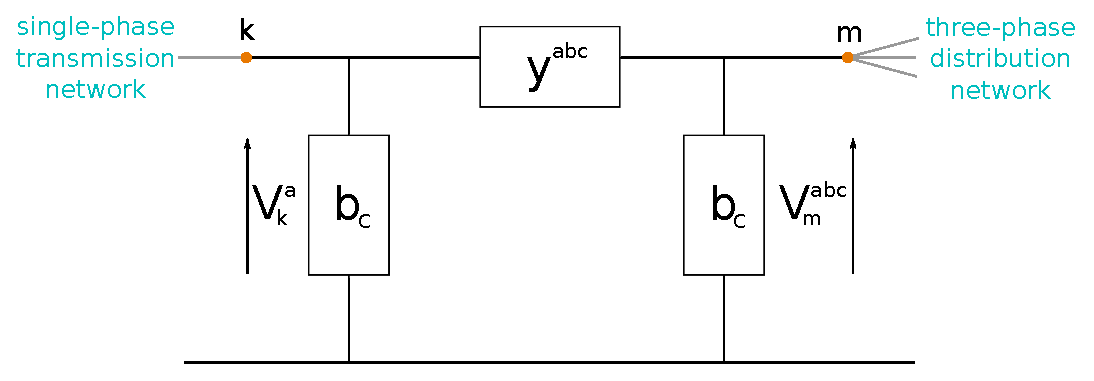
\includegraphics[width=0.8\textwidth]{Images/substationtransformer.eps}
    \caption{The substation transformer in a hybrid network connecting single-phase bus $k$ and three-phase bus $m$.}
    \label{fig:subtrans}
\end{figure}
\label{sect:ic}
The interconnected method is the unified method applied to hybrid networks. A hybrid network consists of a single-phase transmission part and a three-phase distribution part. The substation transformer, between load bus $k$ of the transmission network and the original slack bus $m$ of the distribution network, connects the information between the two networks. It couples the single-phase quantities at the transmission side to the three-phase quantities at distribution side by transforming the nodal admittance matrix $\mathbf{Y}_{km}$. This is depicted in figure \ref{fig:subtrans}. We use three transformer matrices  \begin{equation}
    \mathbf{T_1}, \quad \mathbf{T_3}  = \frac{1}{3}[1\ a\ a^2],\quad \mathbf{T_4}= \frac{1}{3}\left[1 \ 1 \ 1 \right],\quad\mbox{and}\quad \mathbf{T_5}  =\frac{1}{3} \left[1 \ a^2\  a \right],\quad a = e^{\frac{2}{3}\pi\iota},
   \label{eq:T1T2}\nonumber  %= [1\ a^2\ a]^T
\end{equation} to establish the connection of bus $k$ and $m$ via the admittance matrix $\mathbf{Y}_{km}$. This transformation is based on the assumption that the connecting bus $k$ is perfectly balanced. This means that the single-phase and three-phase quantities are related as the following:
\begin{align}
    \begin{bmatrix}V_a & V_b & V_c\end{bmatrix}^T_k &= \mathbf{T_1}\begin{bmatrix}V_a\end{bmatrix}_k,    \label{eq:VA+}
\\
    \begin{bmatrix}I_a\end{bmatrix}_k &= \mathbf{T_3}\begin{bmatrix}I_a & I_b & I_c\end{bmatrix}^T_k,
    \label{eq:IA+}\\
     \begin{bmatrix}S_a\end{bmatrix}_k &= \mathbf{T_4}\begin{bmatrix}S_a & S_b & S_c \end{bmatrix}^T_k.\label{eq:SA+}
\end{align}
The change of the transformer substation depends on whether the unified system is solved using NR-Power or NR-TCIM. The relations \eqref{eq:VA+}, \eqref{eq:IA+}, and \eqref{eq:SA+} are substituted in the corresponding power flow equations. 
\paragraph{Using current injections}
The NR-TCIM method uses Ohm's law directly. The relation between node $k$ and $m$ is expressed as follows:
\begin{align}
    {I}=\mathbf{Y}{V}\quad\Leftrightarrow\quad\begin{bmatrix}
     I_{k} \\
     I_m
    \end{bmatrix} = \begin{bmatrix}
     Y_{11} & Y_{12} \\
     Y_{21} & Y_{22} 
    \end{bmatrix}\begin{bmatrix}
     V_k \\
     V_m
    \end{bmatrix}{}
\end{align}
If node $k$ and $m$ we're both modeled in three-phase, we know the following:
\begin{align}
   {I}_k^{abc}&=\mathbf{Y}^{abc}_{11}{V}_k^{abc}+\mathbf{Y}_{12}^{abc}{V}_m^{abc},\label{eq:IkYV}\\
   {I}_m^{abc}&=\mathbf{Y}^{abc}_{21}{V}_k^{abc}+\mathbf{Y}_{22}^{abc}{V}_m^{abc}.\label{eq:ImYV}
\end{align}
We now multiply equation \eqref{eq:IkYV} by $\mathbf{T_3}$ to obtain $I^a_k$: 
\begin{align}
  I_k^{a} = \mathbf{T_3} \mathbf{I}_k^{abc}&=\mathbf{T_3}\mathbf{Y}^{abc}_{11}{V}_k^{abc}+\mathbf{T_3}\mathbf{Y}_{12}^{abc}\mathbf{V}_m^{abc}.\label{eq:IkTYV}
  \end{align}
We then substitute $\mathbf{V}_k^{abc}$ in equations \eqref{eq:IkTYV} and \eqref{eq:ImYV} by $\mathbf{T_1}V^a_k$ (equation \ref{eq:VA+}): 
\begin{align}
  I_k^{a} = \mathbf{T_3} \mathbf{I}_k^{abc}&=\mathbf{T_3}\mathbf{Y}^{abc}_{11}\mathbf{T_1}V_k^{a}+\mathbf{T_3}\mathbf{Y}_{12}^{abc}\mathbf{V}_m^{abc},\label{eq:IkYVT}\\
    \mathbf{I}_m^{abc}&=\mathbf{Y}^{abc}_{21}\mathbf{T_1}V_k^{a}+\mathbf{Y}_{22}^{abc}{V}_m^{abc}.\label{eq:ImYVT}
\end{align}
From \eqref{eq:IkYVT} and \eqref{eq:ImYVT} we see that our new nodal admittance matrix becomes: 
\renewcommand{\kbldelim}{[}% Left delimiter
\renewcommand{\kbrdelim}{]}% Right delimiter
\begin{align}\mathbf{Y}_{km} =
\kbordermatrix{
& 1 & 3 \\
   1 &  {\mathbf{T_3} [\mathbf{Y}^{abc}_{11}] \mathbf{T_1}} & {\mathbf{T_3} [\mathbf{Y}^{abc}_{12}]}  \\
3 & [\mathbf{Y}^{abc}_{21}]{\mathbf{T_1} } & {\mathbf{Y}^{abc}_{22}} 
  }_{km}
\end{align}
\paragraph{Using power injections}
We can also start from the power equations. The relation between node $k$ and $m$ is expressed as follows: 
\begin{align}
   {S}={V}{I^*}\quad\Leftrightarrow\quad\begin{bmatrix}
     S_{k} \\
     S_m
    \end{bmatrix} = \begin{bmatrix}
     V_k \\
     V_m
    \end{bmatrix}\begin{bmatrix}
    I_k \\
     I_m
    \end{bmatrix}^*
    \end{align}
In the same manner as current injections, we can write this relation in three-phase: 
\begin{align}
   {S}_k^{abc}&={V}_k^{abc}{I}_k^{abc*}+{V}_k^{abc}{I}_m^{abc*},\label{eq:SkYV}\\
   {S}_m^{abc}&={V}_m^{abc}{I}_k^{abc*}+{V}_m^{abc}{I}_m^{abc*}.\label{eq:SmYV} \\
   & \Leftrightarrow \\ 
      {S}_k^{abc}&=\mbox{diag}({V}_k^{abc})\cdot (\mathbf{Y}^{abc}_{kk}{V}_k^{abc})^* +\mbox{diag}({V}_k^{abc})\cdot (\mathbf{Y}^{abc}_{km}{V}_k^{abc})^*,\label{eq:SkYV}\\
   {S}_m^{abc}&=\mbox{diag}({V}_m^{abc})\cdot (\mathbf{Y}^{abc}_{mk}{V}_k^{abc})^* +\mbox{diag}({V}_m^{abc})\cdot (\mathbf{Y}^{abc}_{mm}{V}_m^{abc})^*.\label{eq:SmYV} 
\end{align}
We multiply the first line from the left by $\mathbf{T_4}$ to obtain $S^a_k$: 
\begin{align}
    S_k^a =\mathbf{T_4} S^{abc}_k= \mathbf{T_4} \mbox{diag}({V}_k^{abc})\cdot (\mathbf{Y}^{abc}_{kk}{V}_k^{abc})^* + \mathbf{T_4}\mbox{diag}({V}_k^{abc})\cdot (\mathbf{Y}^{abc}_{km}{V}_m^{abc})^*. \label{eq:STTIChybk}
    \end{align} 
Then, we substitute $V_k^{abc}=\mathbf{T_1}V^a_k$ (equation  \eqref{eq:VA+}) in equations \eqref{eq:SmYV} and \eqref{eq:STTIChybk} and obtain the following:
\begin{align}
    S_k^a &= \mathbf{T_4}\mbox{diag}(\mathbf{T_1}V_k^a)\cdot (\mathbf{Y}_{kk}^{abc}\mathbf{T_1}V_k^a)^* + \mathbf{T_4}\mbox{diag}(\mathbf{T_1}V_k^a)\cdot (\mathbf{Y}_{km}^{abc}V_m^{abc})^*, \label{eq:STIChybk1}\\ 
        S^{abc}_m &=\mbox{diag}(V_m^{abc})\cdot (\mathbf{Y}_{mk}^{abc}\mathbf{T_1}V_k^a)^* + \mbox{diag}(V_m^{abc})\cdot( \mathbf{Y}_{mm}^{abc}V_m^{abc})^*. \label{eq:STIChybm1}
\end{align}
We can rewrite $\mathbf{T_4}\mbox{diag}(\mathbf{T_1}V_k^a)$, the first part of the rhs in \eqref{eq:STIChybk1}, as:
\begin{align}
    \mathbf{T_4}\mbox{diag}(\mathbf{T_1}V_k^a) &\Leftrightarrow \mathbf{T_4}\mbox{diag}(\mathbf{T_1})\mbox{diag}(V_k^a) \\
    &= \frac{1}{3}\begin{bmatrix} 1 & 1 & 1 \end{bmatrix}\begin{bmatrix} 1 &0 &0 \\ 
   0 & a^2 &0 \\ 
    0& 0& a \end{bmatrix}\mbox{diag}(V_k^a) \\
    &\Leftrightarrow\underbrace{\frac{1}{3} \begin{bmatrix}1 & a^2 & a \end{bmatrix}}_{\mathbf{T_5}}\mbox{diag}(V_k^a)\\ 
    &\Leftrightarrow \mbox{diag}(V_k^a) \mathbf{T_5}.\label{eq:VkT6}
\end{align}
This results in the following relations for single-phase and three-phase power: 
\begin{align}
    S_k^a &= \mbox{diag}(V_k^a)\cdot (\mathbf{T_5}\mathbf{Y}_{kk}^{abc}\mathbf{T_1}V_k^a)^* + \mbox{diag}(V_k^a)\cdot (\mathbf{T_5}\mathbf{Y}_{km}^{abc}V_m^{abc})^*, \label{eq:STIChybk}\\ 
        S^{abc}_m &=\mbox{diag}(V_m^{abc})\cdot (\mathbf{Y}_{mk}^{abc}\mathbf{T_1}V_k^a)^* + \mbox{diag}(V_m^{abc})\cdot( \mathbf{Y}_{mm}^{abc}V_m^{abc})^*. \label{eq:STIChybm}
\end{align}
Equations \eqref{eq:STIChybk}, \eqref{eq:STIChybm} yield the following transformed admittance matrix $\mathbf{Y}_{km}$: 
\begin{align}\mathbf{Y}_{km} =
\kbordermatrix{
& 1 & 3 \\
   1 &  {\mathbf{T_5} [\mathbf{Y}^{abc}_{kk}] \mathbf{T_1}} & {\mathbf{T_5} [\mathbf{Y}^{abc}_{km}]}  \\
3 & [\mathbf{Y}^{abc}_{mk}]{\mathbf{T_1} } & {\mathbf{Y}^{abc}_{mm}} 
  }_{km}
\end{align}
\subsection{Manager-Fellow splitting methods}
In contrast to the unified methods, the MFS-methods keep two separate domains, the transmission and distribution network (or the manager and the fellow), and introduces an extra iterative scheme between the domains. The two domains have one overlapping bus: the boundary bus. The boundary bus is the original slack bus of the distribution system and, like the unified methods, can be any load bus of the transmission system. As the two domains are solved separately, the boundary bus remains the slack bus for the distribution system and the load bus for the transmission system. During one MFS-iteration, we solve the fellow, inject the solution of the boundary bus into the manager, and then solve this system. This iterative process continues until the difference between the boundary bus of the two systems is smaller than a certain tolerance value $\epsilon$. As the boundary bus is the slack bus of the distribution system, it requires the voltage $V_B$ as known information. In the first iteration, we initialize the voltage as $V_B=1.0$ pu. In the following iterations, we determine the voltage by solving the transmission system. The boundary bus is a load bus for the transmission system and thus requires the complex power as known. We use the output from the distribution system $S_B$ as input for the transmission system. Algorithm \ref{alg:MFS} shows how the iterative scheme of the MFS-method works.     
\begin{algorithm}
    \caption{General algorithmic approach of the manager-fellow splitting method}
        \label{alg:MFS}
\begin{algorithmic}[1]
        \State Set iteration counter $\nu=0$. Initialize the voltage $V_B^0$ of the fellow.
        \State Solve the distribution system. Output: $S_B^{\nu+1}$.
        \State Inject $S_B^{\nu+1}$ into the manager.
        \State Solve the manager. Output: $V_B^{\nu+1}$.
        \State Is $|V_B^{\nu+1}-V_B^{\nu}|_1 >  \epsilon $ ?  Repeat step 2 till 5.
    \end{algorithmic}
\end{algorithm}
As the MFS-method solves the transmission and distribution systems separately, it allows for using different algorithms per domain. In this way, we choose to solve the distribution system with the advantageous NR-TCIM method and the transmission system with the NR-power method.     \newline\newline
The MFS-method can be applied to homogeneous networks and to hybrid networks. The first one requiring a transformation of the entire manager domain, the latter requiring a transformation of the boundary bus only. 
\subsubsection{{The MFS-homogeneous method}}
The MFS-method applied to homogeneous networks requires a transformation of the single-phase transmission system. The balanced transmission system is transformed in the same was as in the F3P-method. The voltage, power, and admittance of all the buses $i=1,..,N$ are transformed to three-phase equivalents. This idea is summarized in equations \eqref{eq:f3pV} - \eqref{eq:f3pY} of section \ref{sect:f3p}.  

\subsubsection{{The MFS-hybrid method}}
The MFS-method applied to hybrid systems keeps the transmission system in single-phase. Only a transformation of the boundary bus is then required. \newline
As we first solve the distribution system, we receive the complex power $S_B$ as three-phase output, which we have to transform to a single-phase quantity. Once we have solved the transmission system, we have to transform the single-phase output of the voltage $V_B$ of this system. Here again, we assume that the boundary bus $B$ is balanced. Balanced three-phase power in pu is related to single-phase power in \eqref{eq:SA+} according the following relation:
\begin{align}
    [S_a] = \mathbf{T_4}\begin{bmatrix}S_a & S_b & S_c \end{bmatrix}^T, \quad \mathbf{T_4}= \frac{1}{3}\left[1 \ 1 \ 1 \right],\quad\mbox{and}\quad a = e^{\frac{2}{3}\pi\iota}.
\label{eq:MFShS}\end{align}
The voltage of the boundary bus has the same relation as in \eqref{eq:VA+}: 
\begin{align}
    \begin{bmatrix}V_a & V_b & V_c\end{bmatrix}^T_B &= \mathbf{T_1}\begin{bmatrix}V_a\end{bmatrix}_B,\quad 
     \mathbf{T_1} = [1\ a^2\ a]^T,\quad\mbox{and}\quad a = e^{\frac{2}{3}\pi\iota}.\label{eq:MFShV}
    \end{align}
  %  \note{T-1 moet waarschijnlijk a hebben van -23 pi}
The MFS-methods do not require a transformation of the nodal admittance matrix. We transform the necessary boundary parameters directly. At every MFS-iteration, we make transformation \eqref{eq:MFShS} and \eqref{eq:MFShV} after step 2 and step 4 of algorithm \ref{alg:MFS}, respectively. 

\subsubsection{The manager-fellow iterative schemes}
Two iterative schemes of the manager-fellow splitting are defined \cite{Sun2005}. The first is the Convergence Alternating Iterative (CAI) scheme and the other is the Multistep Alternating Iterative (MAI) scheme. In the CAI-scheme, we define an explicit convergence condition for the fellow and for the manager. The fellow is solved with NR-TCIM, for which we define a tolerance value $\epsilon_D$. Once this system has converged, we inject its boundary output into the manager. We solve the manager using NR-power, for which we also define a (not necessarily) different tolerance value $\epsilon_T$. Once the manager has converged, we inject its boundary output into the fellow. The integrated network is converged once we have met the convergence condition of the MFS-algorithm. \\
In the MAI-scheme, we first define a maximum number of iterations per separate system, ie: $I_{max,D}$ and $I_{max,T}$. We inject the output of one system into the other as soon this maximum number of iterations has been reached. The convergence of the integrated network is based on the convergence condition of the MFS-algorithm. 
\paragraph{Speeding up the CAI-scheme} \label{par:caischeme}
We can speed-up the CAI-scheme if we, at every MFS iteration, initialize the voltages as the output of the previous MFS iteration. In the current suggested schemes, we initialize all the buses, except the boundary bus $B$, to $V=1.0$ pu. We can reduce the number of required iterations for the separate systems if we initialize the voltages to its last obtained solution in the previous MFS-iteration, ie: $V^{\nu+1}_{0,D}=V^{\nu}_{I,D}$ and $V^{\nu+1}_{0,T}=V^{\nu}_{I,T}$. 

\subsection{General expectations of the methods} \label{sect:advantages}
Based on the theoretical study of the unified and splitting methods and hybrid and homogeneous networks, we have some first expectations about their performances. Firstly, we expect the methods applied on hybrid networks to perform better in terms of CPU-time. Homogeneous network contain a three-phase representation of the transmission network and thus needs to process a larger Jacobian matrix: If we consider a transmission system with $N$ buses, then the Jacobian matrix of a three-phase network will be of size $6N$ x $6N$ compared to a single-phase Jacobian matrix of size $2N$ x $2N$. Secondly, it is possible that we observe a higher number of iterations for the methods applied on hybrid networks. This expectation is based on the assumption that the connection bus at transmission side is completely balanced while it might be unbalanced due to the connection to the unbalanced distribution system. \\
If we compare the unified and splitting methods, we expect to see an advantage in speed for the unified methods as they only need to solve one system. The splitting methods are advantageous when system operators are not allowed to share complete network information: In the splitting methods, they only need to share information of the connecting boundary bus. 

\newpage 
\section{Numerical assessment}
All previous mentioned methods are implemented into the Matpower\footnote{MATPOWER is a package of free, open-source Matlab-language M-files for solving steady-state power system simulation and optimization problems \cite{Zimmerman2011}} library. Matpower contains several transmission network test cases. The resources page of IEEE Power \& Energy Society contains several distribution network test cases which are all explained in \cite{Schneider2018}. These test cases contain the necessary input to solve power flow problems on separated networks. We created integrated test cases from the existing transmission and distribution test cases. We used the 9-bus, 33-bus, 118-bus, and 3120-bus data as balanced network test cases. All these test-cases except for the 33-bus network are transmission networks. The 33-bus is a balanced distribution network. We use the IEEE 13-bus, 37-bus, 123-bus, and 8500-bus data as unbalanced distribution test cases. We changed the loading of the 37-bus network by shifting 20\% of the original load of phase b equally to phase a and c, like the original authors \cite{Taranto2008} to create an unbalanced network.\\ 
The loads of the IEEE test-networks are connected according the given configuration. The loads in the Matpower test-networks are configured as Wye-P loads in the full three-phase method and the MFS-homogeneous method. The transformers in this method are modeled in a Wye-Wye configuration.
\\ 
We solve the unified methods using NR-TCIM with $\varepsilon=10^{-8}$ as convergence condition. In the splitting methods, we solve the distribution system using NR-TCIM and $\varepsilon_D=10^{-8}$, the transmission system using NR-P and $\varepsilon_T=10^{-8}$, and we define the tolerance value of the MFS-method also as $\varepsilon_{MFS}=10^{-8}$.
\\ \\ 
We created the following integrated test cases by integrating one balanced network to one or multiple unbalanced networks: 
\begin{multicols}{2}
\begin{itemize}
    \item Test case 1: T9-D13
    \item Test case 2: D33-D37
    \item Test case 3: T118-D123
    \item Test case 4: T3120-D8500 
    \item Test case 5: T9-3D13 
    \item Test case 6: T118-3D123 
\end{itemize}
\end{multicols}
\paragraph{Connection bus}
We selected a random load bus in the transmission network as the connection bus in the integrated network. We choose bus $7$ in the 9-bus network, bus $30$ in the 33-bus network, bus $108$ in the 118-bus network, and we choose bus $2700$ in the 3120-bus network. The original reference bus of the distribution network becomes the connection bus at the distribution side of the integrated network. In the unified methods, this former reference bus must be changed to a load bus.  In the splitting method, the distribution reference bus remains a reference bus, initialized by the output it receives from the transmission network. 
Test case 5 and 6 have multiple distribution networks connected. These networks are connected to the mentioned connection bus and its sequential buses. 


\subsection{Results}
In order to solve realistic power flow problems, which are very large electricity networks, we need insight into the speed of the problems. In this section we compare the integration methods on CPU-time and number of iterations. We share the results in table \ref{tab:speed}. 
\begin{table}[h!]
\renewcommand{\arraystretch}{1.3}
\centering
\caption{Comparison on number of iterations (in case of the MFS-method ($I_{MFS}$) and the necessary iterations per subdomain ($I_T$ and $I_D$)), and CPU-time of the integration methods, applied on six test-cases. The top one are methods applied on homogeneous networks. The bottom one is applied on hybrid networks. }\label{tab:speed}
\begin{adjustbox}{width=\textwidth} %, angle=90}
\small
\begin{tabular}{@{}l c cc c  cccc c cccc c  @{}}\toprule
                               && \multicolumn{2}{c}{\textit{F3P}} &&     \multicolumn{4}{c}{\textit{MFS-homo-CAI}} && \multicolumn{4}{c}{\textit{MFS-homo-MAI}} \\ \midrule 
\multicolumn{1}{l}{}        && \textit{its}      & \textit{CPU} && $I_{MFS}$      & $I_T$   &  $I_D$      & \textit{CPU}     &&$I_{MFS}$      & $I_T$   &  $I_D$      & \textit{CPU}      \\
\cmidrule{3-4}  \cmidrule{6-9}  \cmidrule{11-14}   
\multicolumn{1}{c}{test case}      && \textit{\#}       & \textit{sec} && \textit{\#}      & \textit{\#}    & \textit{\#}       & \textit{sec}     && \textit{\#}        & \textit{\#}     &  \textit{\#}       & \textit{sec}  \\
\midrule
\multicolumn{1}{c}{\textit{T9-D13 (7)}}           && 4  & {0.018}    && 4  & 4 & 5 &  \textbf{1.37} && 4  & 4 & 5 & {1.44}\\
\multicolumn{1}{c}{\textit{D33-D37 (30)}}         && 4  & {0.018}    && 18 & 3 & 5 &  \textbf{6.15} && 18  & 3 & 4  & {6.32}\\
\multicolumn{1}{c}{{\textit{T118-D123 (108)}}}    && 6  & {0.041}    && 3  & 4 & 5 &  \textbf{1.25} && -  &  &  &    \\
\multicolumn{1}{c}{{\textit{T3120-D8500 (2700)}}} && 5  & {0.521}    && 3  & 6 & 5 &  \textbf{3.71} && -  &  &  &  \\
\multicolumn{1}{c}{{\textit{T9-3D13 (7-9)}}}      && 4  & {0.023}    && 4  & 4 & 5 &  \textbf{2.38} && -  &  &  &      \\
 \multicolumn{1}{l}{\textit{T118-3D123} (108-110)}          && 13 & {0.127}    && 3  & 4 & 4 &  \textbf{2.43} && -  &  & \textbf{-} \\
% \multicolumn{1}{l}{{\textit{T9-3D13}}}    && - & - && - & -    && -       & - & -  & \textbf{-} && -   & - & - &  - && -       & -  & - & - && -       & -  & - & - \\
\toprule 
\end{tabular}
\end{adjustbox}
%homogeneous
\begin{adjustbox}{width=1\textwidth} %, angle=90}
\small
\begin{tabular}{@{}l c cc c  cccc c cccc c  @{}}\toprule
                               && \multicolumn{2}{c}{\textit{IC}} &&     \multicolumn{4}{c}{\textit{MFS-hybrid-CAI}} && \multicolumn{4}{c}{\textit{MFS-hybrid-MAI}} \\ \midrule 
\multicolumn{1}{l}{}        && \textit{its}      & \textit{CPU} && $I_{MFS}$      & $I_T$   &  $I_D$      & \textit{CPU}     &&$I_{MFS}$      & $I_T$   &  $I_D$      & \textit{CPU}      \\
\cmidrule{3-4}  \cmidrule{6-9}  \cmidrule{11-14}   
\multicolumn{1}{c}{test case}      && \textit{\#}       & \textit{sec} && \textit{\#}      & \textit{\#}    & \textit{\#}       & \textit{sec}     && \textit{\#}        & \textit{\#}     &  \textit{\#}       & \textit{sec}  \\
\midrule
\multicolumn{1}{c}{\textit{T9-D13 (7)}}           && 4  & {0.013}    && 4  & 4 & 5 &  1.02 && 4  & 4 & 5 & {1.02}\\
\multicolumn{1}{c}{\textit{D33-D37 (30)}}         && 4  & {0.021}    && 18 & 3 & 5 &  4.41 && 18  & 3 &  4 & {4.36}\\
\multicolumn{1}{c}{{\textit{T118-D123 (108)}}}    && 8  & {0.039}    && 3  & 7 & 6 &  1.01 && -  &  &  &    \\
\multicolumn{1}{c}{{\textit{T3120-D8500 (2700)}}} && 5  & {0.288}    && 3  & 6 & 5 &  2.44 && -  &  &  &  \\
\multicolumn{1}{c}{{\textit{T9-3D13 (7-9)}}}      && 5  & {0.019}    && 4  & 4 & 5 &  2.02 && -  &  &  &      \\
 \multicolumn{1}{l}{\textit{T118-3D123 (108-110)}}          && 10 & 0.126    && 3  & 7 & 8 &  2.18 && -  &  & \textbf{-} \\
% \multicolumn{1}{l}{{\textit{T9-3D13}}}    && - & - && - & -    && -       & - & -  & \textbf{-} && -   & - & - &  - && -       & -  & - & - && -       & -  & - & - \\
\toprule 
\end{tabular}
\end{adjustbox}
\end{table}

%\begin{table}[h]
\renewcommand{\arraystretch}{1.3}
\centering
\caption{Comparison on number of iterations (in case of the MSS-method ($I_{MSS}$) and the necessary iterations per subdomain ($I_T$ and $I_D$)), and CPU-time of the integration methods, applied on five test-cases. The top one are methods applied on homogeneous networks. The bottom one is applied on hybrid networks. }\label{tab:speed}
\begin{adjustbox}{width=1\textwidth} %, angle=90}
\small
\begin{tabular}{@{}l c cc c  cccc c cccc c  @{}}\toprule
                               && \multicolumn{2}{c}{\textit{F3P}} &&     \multicolumn{4}{c}{\textit{MS-homo-CAI}} && \multicolumn{4}{c}{\textit{MS-homo-MAI}} \\ \midrule 
\multicolumn{1}{l}{}        && \textit{its}      & \textit{CPU} && $I_{MSS}$      & $I_T$   &  $I_D$      & \textit{CPU}     &&$I_{MSS}$      & $I_T$   &  $I_D$      & \textit{CPU}      \\
\cmidrule{3-4}  \cmidrule{6-9}  \cmidrule{11-14}   
\multicolumn{1}{c}{test case}      && \textit{\#}       & \textit{sec} && \textit{\#}      & \textit{\#}    & \textit{\#}       & \textit{sec}     && \textit{\#}        & \textit{\#}     &  \textit{\#}       & \textit{sec}  \\
\midrule
\multicolumn{1}{c}{\textit{T9-D13 (7)}}         && 4 &\textbf{ 0.610}    && 4 & 4 & 4 &  0.237 && 6 & 2 & 2  & {0.257}\\
\multicolumn{1}{c}{\textit{T9-D37 (7)}}         && 4 & \textbf{0.587}    && 3 & 4 & 4 &  0.262 && 6 & 2 & 2  & {0.299}\\
\multicolumn{1}{c}{{\textit{T118-D13 (118)}}}   && 5 & \textbf{0.763}    && 3 & 7 & 5  & 0.324 && 4 & 2 & 2 &  0.297  \\
\multicolumn{1}{c}{{\textit{T118-D37 (118)}}}   && 5 & \textbf{0.920}    && 3 & 7 & 5  & 0.360 && 3 & 4 & 4 &  0.3253\\
\multicolumn{1}{c}{{\textit{T3120-D37 (3003)}}} && 5 & \textbf{2438}     && 3 & 6 & 4  & 1213  && 6 & 2 & 2 &  841    \\
% \multicolumn{1}{l}{\textit{T9-2D13}}       && - & - && - & -    && -       & - & -  & \textbf{-} && -   & - & - &  - && -       & -  & - & - && -       & -  & - & - \\
% \multicolumn{1}{l}{{\textit{T9-3D13}}}    && - & - && - & -    && -       & - & -  & \textbf{-} && -   & - & - &  - && -       & -  & - & - && -       & -  & - & - \\
\toprule 
\end{tabular}
\end{adjustbox}
%homogeneous
\begin{adjustbox}{width=1\textwidth} %, angle=90}
\small
\begin{tabular}{@{}l c cc c  cccc c cccc c  @{}}\toprule
                               && \multicolumn{2}{c}{\textit{IC}} &&     \multicolumn{4}{c}{\textit{MS-hybrid-CAI}} && \multicolumn{4}{c}{\textit{MS-hybrid-MAI}} \\ \midrule 
\multicolumn{1}{l}{}        && \textit{its}      & \textit{CPU} && $I_{MSS}$      & $I_T$   &  $I_D$      & \textit{CPU}     &&$I_{MSS}$      & $I_T$   &  $I_D$      & \textit{CPU}      \\
\cmidrule{3-4}  \cmidrule{6-9}  \cmidrule{11-14}   
\multicolumn{1}{c}{test case}      && \textit{\#}       & \textit{sec} && \textit{\#}      & \textit{\#}    & \textit{\#}       & \textit{sec}     && \textit{\#}        & \textit{\#}     &  \textit{\#}       & \textit{sec}  \\
\midrule
\multicolumn{1}{c}{\textit{T9-D13 (7)}}          && 4 & {0.455 } && 4      & 4  & 4 & 0.308 && 6     & 2  & 2 & 0.323  \\
\multicolumn{1}{c}{\textit{T9-D37 (7)}}          && 4 & 0.464    && 3      & 4  & 4 & 0.325 && 6     & 2  & 2 & 0.352  \\
\multicolumn{1}{c}{{\textit{T118-D13 (118)}}}    && 4 & 0.522    && 3      & 7  & 5 & 0.348 && 4     & 2  & 2 & {0.312} \\
\multicolumn{1}{c}{{\textit{T118-D37 (118)}}}    && 4 & 0.518    && 3      & 7  & 5 & 0.356 && 3     & 4  & 4 & {0.353}\\
\multicolumn{1}{c}{{\textit{T3120-D37 (3003)}}}  && 5 & 143      && 3      & 6  & 4 & 383   && 6     & 2  & 2 & {235}  \\
% \multicolumn{1}{l}{\textit{T9-2D13}}       && - & - && - & -    && -       & - & -  & \textbf{-} && -   & - & - &  - && -       & -  & - & - && -       & -  & - & - \\
% \multicolumn{1}{l}{{\textit{T9-3D13}}}    && - & - && - & -    && -       & - & -  & \textbf{-} && -   & - & - &  - && -       & -  & - & - && -       & -  & - & - \\
\toprule 
\end{tabular}
\end{adjustbox}
\end{table}
\begin{figure}
    \centering
    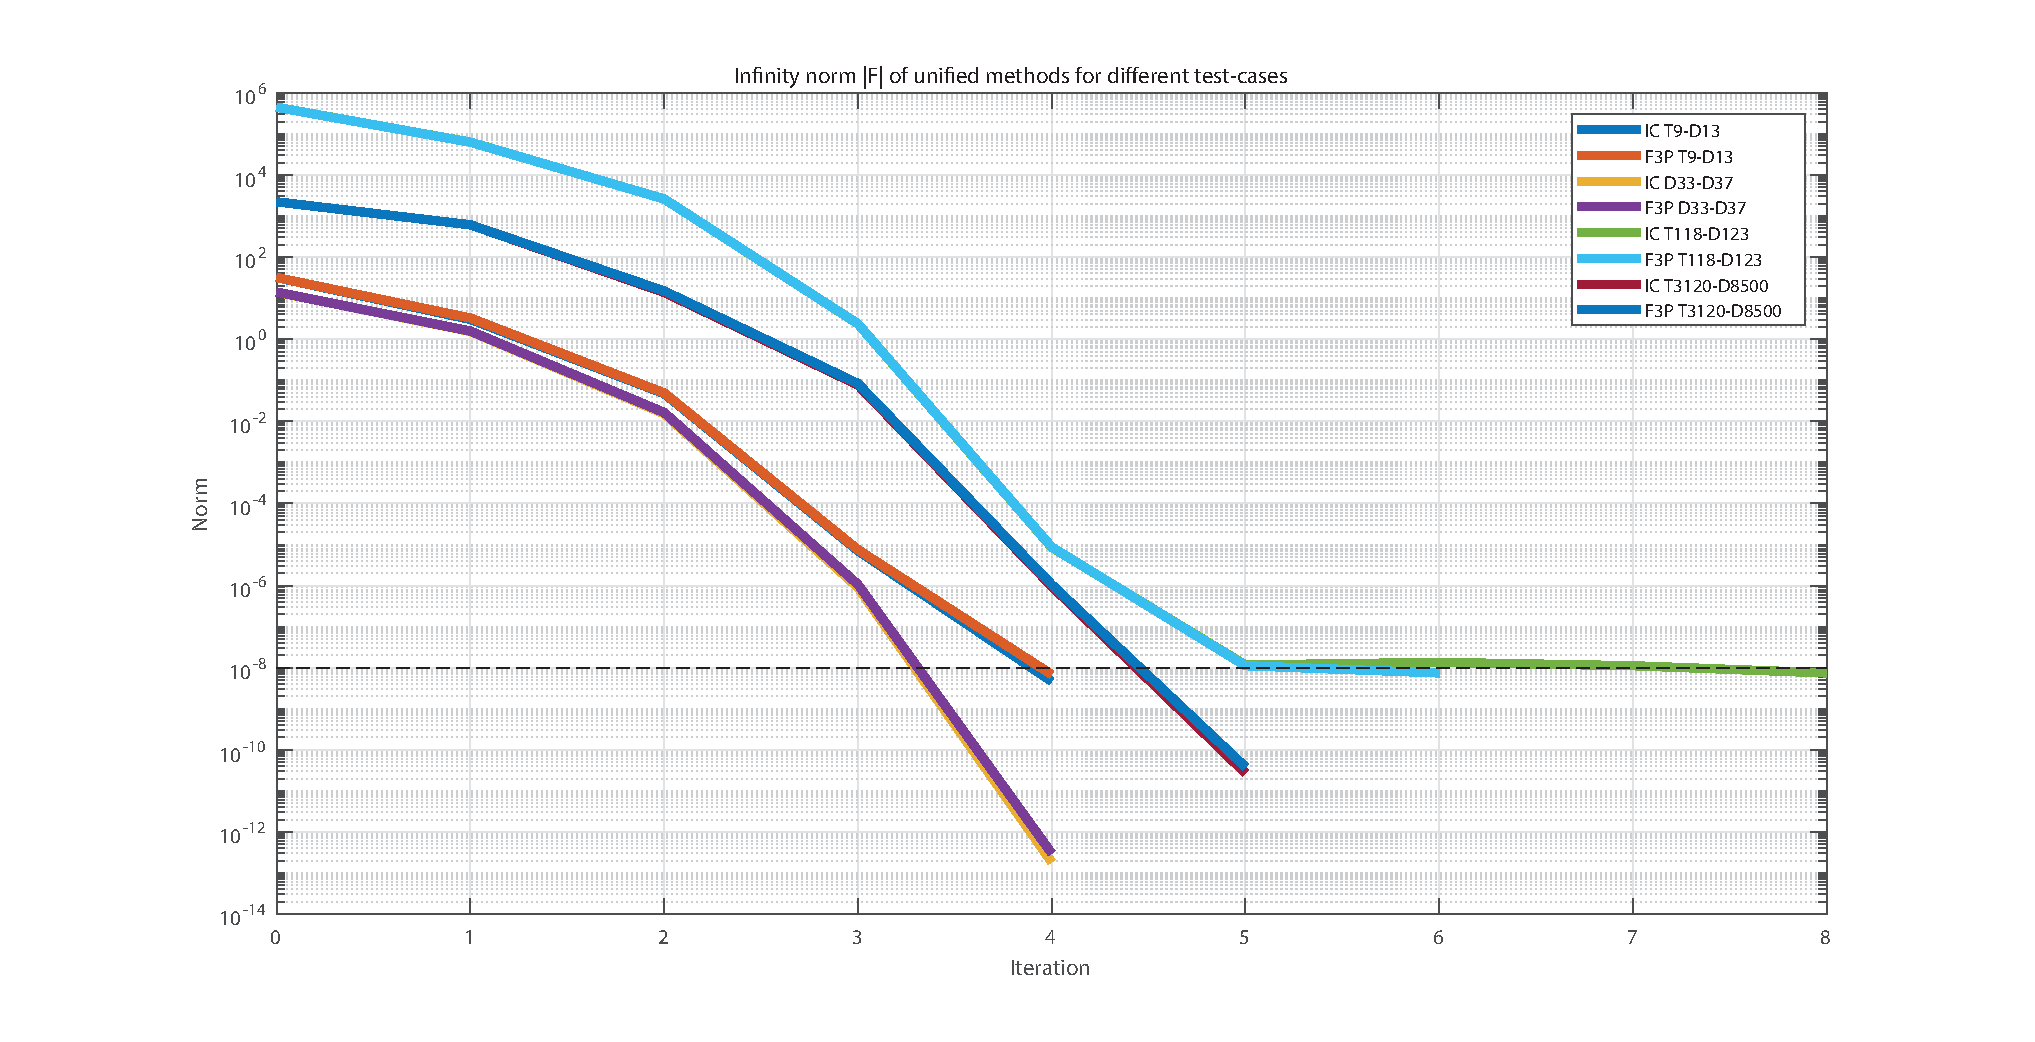
\includegraphics[width=\textwidth]{Images/unifiednorms.eps}
    \caption{Plots of $|F|_\infty$ of the unified methods for four different test-cases. The black dotted line is the tolerance value, ie $\epsilon=1e-8$.}
    \label{fig:uninorm}
\end{figure}
\begin{figure}
    \centering
    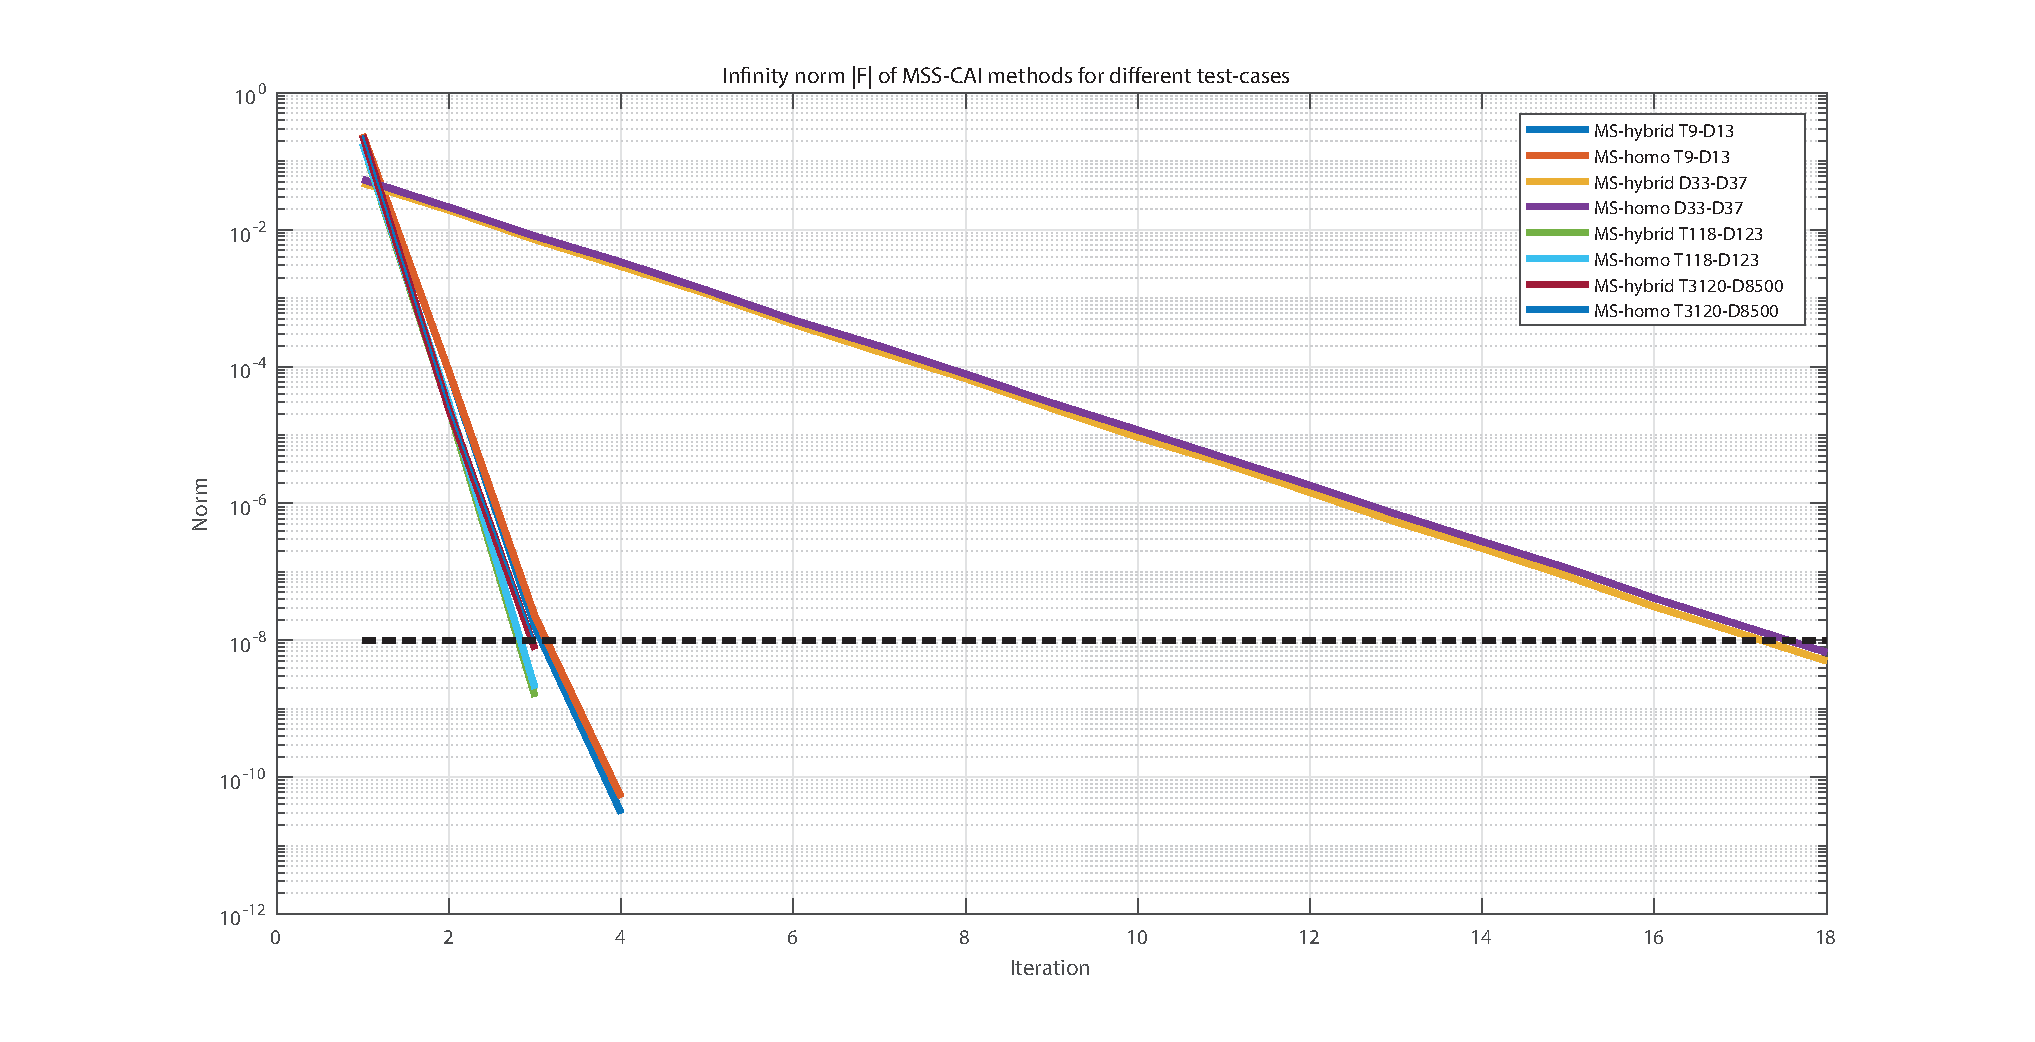
\includegraphics[width=\textwidth]{Images/MSSCAInorms.eps}
    \caption{Plots of $|V_B^{\nu+1}-V_B^{\nu}|_\infty$ of the splitting methods for four different test-cases. The black dotted line is the tolerance value, ie $\epsilon=1e-8$.}
    \label{fig:MFSnorm}
\end{figure}
\noindent These results show that over all the test cases, the MFS-homo method performs the least\todo{I stopped using the MAI-scheme, because it is either not converging or producing the exact same results as the CAI-scheme. Either I include this as a note or we completely disregard the MAI-scheme in the report }. The unified methods are are comparable in speed for the small test-cases. The big test case, T3120-D8500, gives the most significant results. The hybrid network methods are a lot faster than the homogeneous methods. \newline \newline
There is not a clear significance in the results of the MFS-CAI- and MAI-schemes. We recommend to use the CAI-schemes as with the MAI-schemes you first have to determine the number subiterations that is are required to reach convergence. Then, you will get very similar results as in the CAI-scheme but with an extra preprocessing step.  

\section{Conclusion}
We have reviewed and assessed two types of integration methods to solve the power flow problem. We classified them as unified and splitting methods and applied them on hybrid and homogeneous networks. The splitting methods could be further divided in two different iterating schemes. This resulted in six different methods as starting point of our numerical comparison study. We investigated if the methods produced accurate results and analyzed the speed and number of iterations to reach convergence. \newline
From this assessment we can conclude that the unified methods are most favorable in sense of CPU-time compared to splitting methods, in line with the expectations we stated in section \ref{sect:advantages}. The differences within the unified methods are less significant than we expected. We argued that the increase in size of the Jacobian would have resulted in increase of CPU-time. Only in the bigger test-case T3120-D8500 that the difference becomes significant: The F3P-method is around twice as slow as the Interconnected method. \newline 
Based on these results we would recommend to choose the unified methods applied on hybrid networks when this is possible. But in geographically distinct locations, or when legislation prohibits system operators to share complete network data, the splitting methods are a good alternative. The speed of the CAI-schemes can be reduced if we apply the idea of paragraph \ref{par:caischeme}. \newline\newline
The next step is to continue with realistic test cases which can be up to millions of buses per network domain. In most countries, the real transmission network is much smaller than the distribution network and a country has in general more than one distribution network. The differences between homogeneous and hybrid methods then become less significant.  To solve these very large systems in reasonable amount of time, we have to adapt the methods, using Newton-Krylov methods and preconditioning techniques  \cite{Idema2013}, for a parallel or GPU environment. Then, the MFS-hybrid-CAI method gets the advantage when multiple distribution networks are connected to one transmission network as it is a domain-decomposition approach: multiple distribution networks can run on parallel cores. Doing new simulations using these speed-up techniques on realistically sized networks, should give a better idea which method is most favorable to solve the integrated power flow problem. 

%\section{References}
\newpage
\bibliographystyle{ieeetr}
\bibliography{pscc3} 
%\subsubsection{Accuracy} 
To check the accuracy of the methods, we compare the voltage output of the integrated methods with the output of the separated methods. We solve the transmission network separately using NR-power and we solve the distribution network separately using NR-TCIM. The distribution domain in the integrated network has no reference bus anymore. In order to compare the voltage profile of this part, we scale the values accordingly. 
We know that the voltage is given by: \begin{equation}
V_p=|V|_p\exp{(\iota\delta_{V_p}-\phi)},\quad p\in\{a,b,c\},
\end{equation}
where $|V|$ and $\delta$ are set to $|V|=1.0$ pu and $\delta=0$ at the reference bus. We can compare the voltage of the distribution domain to the voltage of the separated domain after scaling. We divide the voltage magnitude of the distribution domain, buses $i=1,...,N_D$, by the voltage magnitude of the distribution connection bus: 
\begin{equation}
|V|_{i,{D_{new}}} = \frac{|V|_{i,{D_{uns}}}}{|V|_{ref,{D_{uns}}}},\quad i=1,..,N_D.
\label{eq:ViDnew}
\end{equation}
The subscript $uns$ represents the unscaled values and $new$ represents the scaled values. \newline 
The voltage angle represents the phase-shift in relation to the phase of the reference bus. In order to compare the integrated output of the voltage angle with the separated output, we subtract the phase-angle of the former reference bus from all the buses $i=1,..,N_D$: 
\begin{equation}
\delta_{i,{D_{new}}} ={\delta_{i,{D_{uns}}}}-{\delta_{ref,{D_{uns}}}},\quad i=1,..,D_N.
\label{eq:dViDnew}
\end{equation}
Note that we need to apply \eqref{eq:ViDnew} and \eqref{eq:dViDnew} to all the three phases separately. \newline\newline
We compare the voltage magnitudes and angles of the integrated network, including the scaled distribution domain, with the magnitudes angles of the separate domains. We take the infinity norm of the relative difference between the voltages: 
\begin{equation}
\mbox{rel. error of } |V|_p = \left|\frac{|V|^*_p - |V|^o_p}{|V|^o_p}\right|_\infty,\quad p\in\{a,b,c\},
\label{eq:norm|V|}
\end{equation}
where the asterisk $*$ marks the outcome of separated networks, and the superscript $o$ the output of separated networks (o=original). We do this in a similar manner for the voltage angle: 
\begin{equation}
\mbox{rel. error of } \delta_p = \left|\frac{\delta^*_p - \delta^o_p}{\delta^o_p}\right|_\infty,\quad p\in\{a,b,c\},
\label{eq:normdelta}
\end{equation}
We have given the relative errors of the voltage magnitude and angle of the three phases for all the test cases in table \ref{tab:relerror}. 

\begin{table}[h]
\renewcommand{\arraystretch}{1.3}
\centering
\caption{Relative error of the voltage magnitude and angle of the three phases for all the integration methods. }\label{tab:relerror}
\begin{adjustbox}{width=1\textwidth} %, angle=90}
\small
\begin{tabular}{ccccccccc}
\toprule
{} && \multicolumn{7}{c}{Full three-phase}   \\
\cmidrule{3-9}
{} && \multicolumn{3}{c}{$|V|$} && \multicolumn{3}{c}{$\delta$}  \\
\cmidrule{3-5}\cmidrule{7-9}
 test case &&        a &        b &       c &&        a &       b &        c \\
\midrule
T9-D13    &&  3.854e-04 &  6.851e-04 &  2.000e-04 &&  -6.119e-03 &  -5.376e-03 &  -6.475e-03 \\
T9-D37    &&  4.000e-04 &  5.153e-04 &  4.100e-04 &&   3.769e-01 &  -1.230e-02 &   1.529e-01 \\
T118-D37  &&  9.791e-05 &  6.000e-05 &  7.000e-05 &&   3.979e-01 &   3.600e-01 &   4.237e-01 \\
T3120-D37 &&  2.409e-04 &  7.524e-04 &  1.293e-04 &&   2.271e+00 &   2.121e-01 &   2.495e-01 \\
\bottomrule
\end{tabular}
\end{adjustbox}
%N2I1

\begin{adjustbox}{width=1\textwidth} %, angle=90}
\small
\begin{tabular}{ccccccccc}
\toprule
{test case} && \multicolumn{7}{c}{MSS-homo-CAI}   \\
%\cmidrule{3-9}
%{} && \multicolumn{3}{c}{$|V|$} && \multicolumn{3}{c}{$\delta$}  \\
%\cmidrule{3-5}\cmidrule{7-9}
 %test-case &&        a &        b &       c &&        a &       b &        c \\
\midrule
T9-D13       &&  2.934e-04 &  7.982e-04 &  2.874e-04 &&  4.794e-02 &  4.246e-02 &  5.097e-02 \\
T9-D37       &&  1.916e-04 &  5.394e-04 &  1.916e-04 &&  2.271e+00 &  1.571e-02 &  3.297e-02 \\
T118-D37     &&  8.984e-03 &  8.911e-03 &  9.005e-03 &&  4.501e-01 &  4.468e-01 &  4.524e-01 \\
T3120-D37    &&  2.440e-04 &  7.296e-04 &  1.303e-04 &&  3.434e-01 &  1.951e-02 &  4.082e-02 \\
%MaxT9-D13    &&         14 &         16 &          6 &&          3 &          3 &          3 \\
%MaxT9-D37    &&          6 &         41 &          6 &&         23 &          3 &          3 \\
%MaxT118-D37  &&        117 &        117 &        117 &&         92 &         92 &         92 \\
%MaxT3120-D37 &&       3137 &       3152 &       3126 &&       3133 &       2017 &       2017 \\
\bottomrule
\end{tabular}
\end{adjustbox}
%N2I2
\begin{adjustbox}{width=1\textwidth} %, angle=90}
\small
\begin{tabular}{ccccccccc}
\toprule
{test case} && \multicolumn{7}{c}{MSS-homo-MAI, 2 iterations per subdomain}   \\
%\cmidrule{3-9}
%{} && \multicolumn{3}{c}{$|V|$} && \multicolumn{3}{c}{$\delta$}  \\
%\cmidrule{3-5}\cmidrule{7-9}
% test-case &&        a &        b &       c &&        a &       b &        c \\
\midrule
T9-D13       &&  5.749e-04 &  7.037e-04 &  5.749e-04 &&  6.702e-02 &  1.231e+00 &  1.261e+00 \\
T9-D37       &&  4.364e-04 &  4.796e-04 &  3.958e-04 &&  2.587e+01 &  2.724e-02 &  1.011e+01 \\
T118-D37     &&  2.017e-01 &  2.017e-01 &  2.017e-01 &&  1.993e+01 &  1.993e+01 &  1.993e+01 \\
T3120-D37    &&  1.048e-01 &  1.048e-01 &  1.048e-01 &&  4.504e+02 &  1.535e+01 &  8.085e+01 \\
%MaxT9-D13    &&          6 &         16 &          6 &&          8 &         11 &         11 \\
%MaxT9-D37    &&          8 &         19 &          8 &&         22 &          8 &         31 \\
%MaxT118-D37  &&         82 &         82 &         82 &&         92 &         92 &         92 \\
%MaxT3120-D37 &&         32 &         32 &         32 &&       3134 &       2009 &       3128 \\
\bottomrule
\end{tabular}
\end{adjustbox}
%IC
%\label{}\hspace{2cm}%\caption{Relative error of the voltage magnitude and angle of the three phases obtained using the interconnected method. }
\begin{adjustbox}{width=1\textwidth} %, angle=90}
\small
\begin{tabular}{ccccccccc}
\toprule
{test case} && \multicolumn{7}{c}{Interconnected}   \\
%\cmidrule{3-9}
%{} && \multicolumn{3}{c}{$|V|$} && \multicolumn{3}{c}{$\delta$}  \\
%\cmidrule{3-5}\cmidrule{7-9}
% test-case &&        a &        b &       c &&        a &       b &        c \\
\midrule
T9-D13    &&  2.895e-04 &  6.851e-04 &  2.000e-04 &&  -6.000e-03 &  -6.000e-03 &  -6.000e-03 \\
T9-D37    &&  4.000e-04 &  5.247e-04 &  4.000e-04 &&   3.769e-01 &   3.769e-01 &   3.769e-01 \\
T118-D37  &&  9.791e-05 &  7.000e-05 &  7.000e-05 &&   3.939e-01 &   3.939e-01 &   3.939e-01 \\
T3120-D37 &&  2.409e-04 &  7.180e-04 &  1.593e-04 &&   3.434e-01 &   2.320e-01 &   2.320e-01 \\
\bottomrule
\end{tabular}
\end{adjustbox}

%N1I1
\begin{adjustbox}{width=1\textwidth} %, angle=90}
\small
\begin{tabular}{ccccccccc}
\toprule
{test case} && \multicolumn{7}{c}{MSS-hybrid-CAI}   \\
%\cmidrule{3-9}
%{} && \multicolumn{3}{c}{$|V|$} && \multicolumn{3}{c}{$\delta$}  \\
%\cmidrule{3-5}\cmidrule{7-9}
% test-case &&        a &        b &       c &&        a &       b &        c \\
\midrule
T9-D13       &&  2.934e-04 &  7.982e-04 &  2.874e-04 &&  4.712e-02 &  4.712e-02 &  4.712e-02 \\
T9-D37       &&  1.916e-04 &  5.299e-04 &  1.916e-04 &&  3.434e-01 &  2.487e-02 &  1.529e-01 \\
T118-D37     &&  8.963e-03 &  8.963e-03 &  8.963e-03 &&  4.497e-01 &  4.497e-01 &  4.497e-01 \\
T3120-D37    &&  2.440e-04 &  7.296e-04 &  1.303e-04 &&  2.271e+00 &  3.085e-02 &  1.529e-01 \\
%MaxT9-D13    &&         14 &         16 &          6 &&          3 &          3 &          3 \\
%MaxT9-D37    &&          6 &         40 &          6 &&         22 &          3 &         17 \\
%MaxT118-D37  &&        117 &        117 &        117 &&         92 &         92 &         92 \\
%MaxT3120-D37 &&       3137 &       3152 &       3126 &&       3134 &       2017 &       3128 \\
\bottomrule
\end{tabular}
\end{adjustbox}

%N1I2
\begin{adjustbox}{width=1\textwidth} %, angle=90}
\small
\begin{tabular}{ccccccccc}
\toprule
{test case} && \multicolumn{7}{c}{MSS-hybrid-MAI, 2 iterations per subdomain}   \\
%\cmidrule{3-9}
%{} && \multicolumn{3}{c}{$|V|$} && \multicolumn{3}{c}{$\delta$}  \\
%\cmidrule{3-5}\cmidrule{7-9}
% test-case &&        a &        b &       c &&        a &       b &        c \\
\midrule
T9-D13       &&  5.749e-04 &  7.037e-04 &  5.749e-04 &&  6.932e-02 &  1.295e+00 &  1.261e+00 \\
T9-D37       &&  4.262e-04 &  5.400e-04 &  4.262e-04 &&  2.721e+01 &  3.459e-02 &  1.011e+01 \\
T118-D37     &&  2.017e-01 &  2.017e-01 &  2.017e-01 &&  1.993e+01 &  1.993e+01 &  1.993e+01 \\
T3120-D37    &&  1.048e-01 &  1.048e-01 &  1.048e-01 &&  4.504e+02 &  1.536e+01 &  8.085e+01 \\
%MaxT9-D13    &&          6 &         16 &          6 &&          8 &         11 &         11 \\
%MaxT9-D37    &&          8 &         41 &          8 &&         22 &          8 &         31 \\
%MaxT118-D37  &&         82 &         82 &         82 &&         92 &         92 &         92 \\
%MaxT3120-D37 &&         32 &         32 &         32 &&       3134 &       2009 &       3128 \\
\bottomrule
\end{tabular}
\end{adjustbox}
\end{table}
\paragraph{The MAI-scheme}
Table \ref{tab:relerror} shows that all the integration methods produce accurate results, except for the MSS-homo-MAI and MSS-hybrid-MAI methods. This is caused by the number of iterations per subdomain that has been set too low. To produce more accurate results, we increased the number of iterations per subdomain simultaneously. We started with $I_{T,max}=I_{D,max}=2$ until $I_{T,max}=I_{D,max}=6$.  Table \ref{tab:MAIschemes} shows the results. Next to the relative error, this table shows the required number of MSS iterations and how long it takes to reach convergence. We only applied these tests on test case T118-D37, as these results were least accurate. When using $4$ iterations per subdomain, the results become as accurate as the MSS-CAI methods. 
\begin{table}[h]
\renewcommand{\arraystretch}{1.3}
\centering
\caption{The relative error of the voltage of test case T118-D37, solved using the MAI-iterative scheme with increasing number of subiterations, $I_T, I_D$, applied on a homogeneous network (top) and on a hybrid network (bottom).}\label{tab:MAIschemes}
\begin{adjustbox}{width=1\textwidth} %, angle=90}
\small
\begin{tabular}{cccccccccccc}
\toprule
{} && \multicolumn{7}{c}{MSS-homo-MAI} && &  \\
\cmidrule{3-9}
{} && \multicolumn{3}{c}{$|V|$} && \multicolumn{3}{c}{$\delta$} && \\
\cmidrule{3-5}\cmidrule{7-9}
{$I_T$,$I_D$} &&        a &        b &       c &&        a &       b &        c && sec & $I_{MSS}$\\
\midrule
2 &&  2.017e-01 &  2.017e-01 &  2.017e-01 &&  1.993e+01 &  1.993e+01 &  1.993e+01 && 0.325 & 4 \\
3 &&  3.436e-02 &  3.436e-02 &  3.436e-02 &&  7.153e+00 &  7.150e+00 &  7.156e+00 && 0.368 & 5 \\
4 &&  9.069e-03 &  9.005e-03 &  9.100e-03 &&  7.426e-01 &  7.393e-01 &  7.448e-01 && 0.323 & 3\\
5 &&  8.984e-03 &  8.911e-03 &  9.005e-03 &&  4.507e-01 &  4.474e-01 &  4.530e-01 && 0.351 & 3\\
6 &&  8.984e-03 &  8.911e-03 &  9.005e-03 &&  4.501e-01 &  4.468e-01 &  4.524e-01 && 0.347 & 3\\
\bottomrule
\end{tabular}
\end{adjustbox}
%N1 
\begin{adjustbox}{width=1\textwidth} %, angle=90}
\small
\begin{tabular}{cccccccccccc}
\toprule
{} && \multicolumn{7}{c}{MSS-hybrid-MAI} && &  \\
\cmidrule{3-9}
{} && \multicolumn{3}{c}{$|V|$} && \multicolumn{3}{c}{$\delta$} && \\
\cmidrule{3-5}\cmidrule{7-9}
{$I_T$,$I_D$} &&        a &        b &       c &&        a &       b &        c && sec & $I_{MSS}$\\
\midrule
2 &&  2.017e-01 &  2.017e-01 &  2.017e-01 &&  1.993e+01 &  1.993e+01 &  1.993e+01 && 0.358 & 4 \\
3 &&  3.436e-02 &  3.436e-02 &  3.436e-02 &&  7.153e+00 &  7.153e+00 &  7.153e+00 && 0.380& 5\\
4 &&  9.058e-03 &  9.058e-03 &  9.058e-03 &&  7.422e-01 &  7.422e-01 &  7.422e-01 && 0.353& 3\\
5 &&  8.963e-03 &  8.963e-03 &  8.963e-03 &&  4.504e-01 &  4.504e-01 &  4.504e-01 && 0.354& 3 \\
6 &&  8.963e-03 &  8.963e-03 &  8.963e-03 &&  4.497e-01 &  4.497e-01 &  4.497e-01 && 0.351&3\\
\bottomrule
\end{tabular}
\end{adjustbox}

\end{table}

We plotted the voltage magnitude and angles of the MAI-schemes to show how the solution, with every increase of the maximum number of subiterations, approaches its `true' results. For comparison we plotted the separated transmission and distribution network as `true' solution in figures \ref{fig:MAIN2} - \ref{fig:ZMAIN1}. 

\begin{figure}[h]
\centering
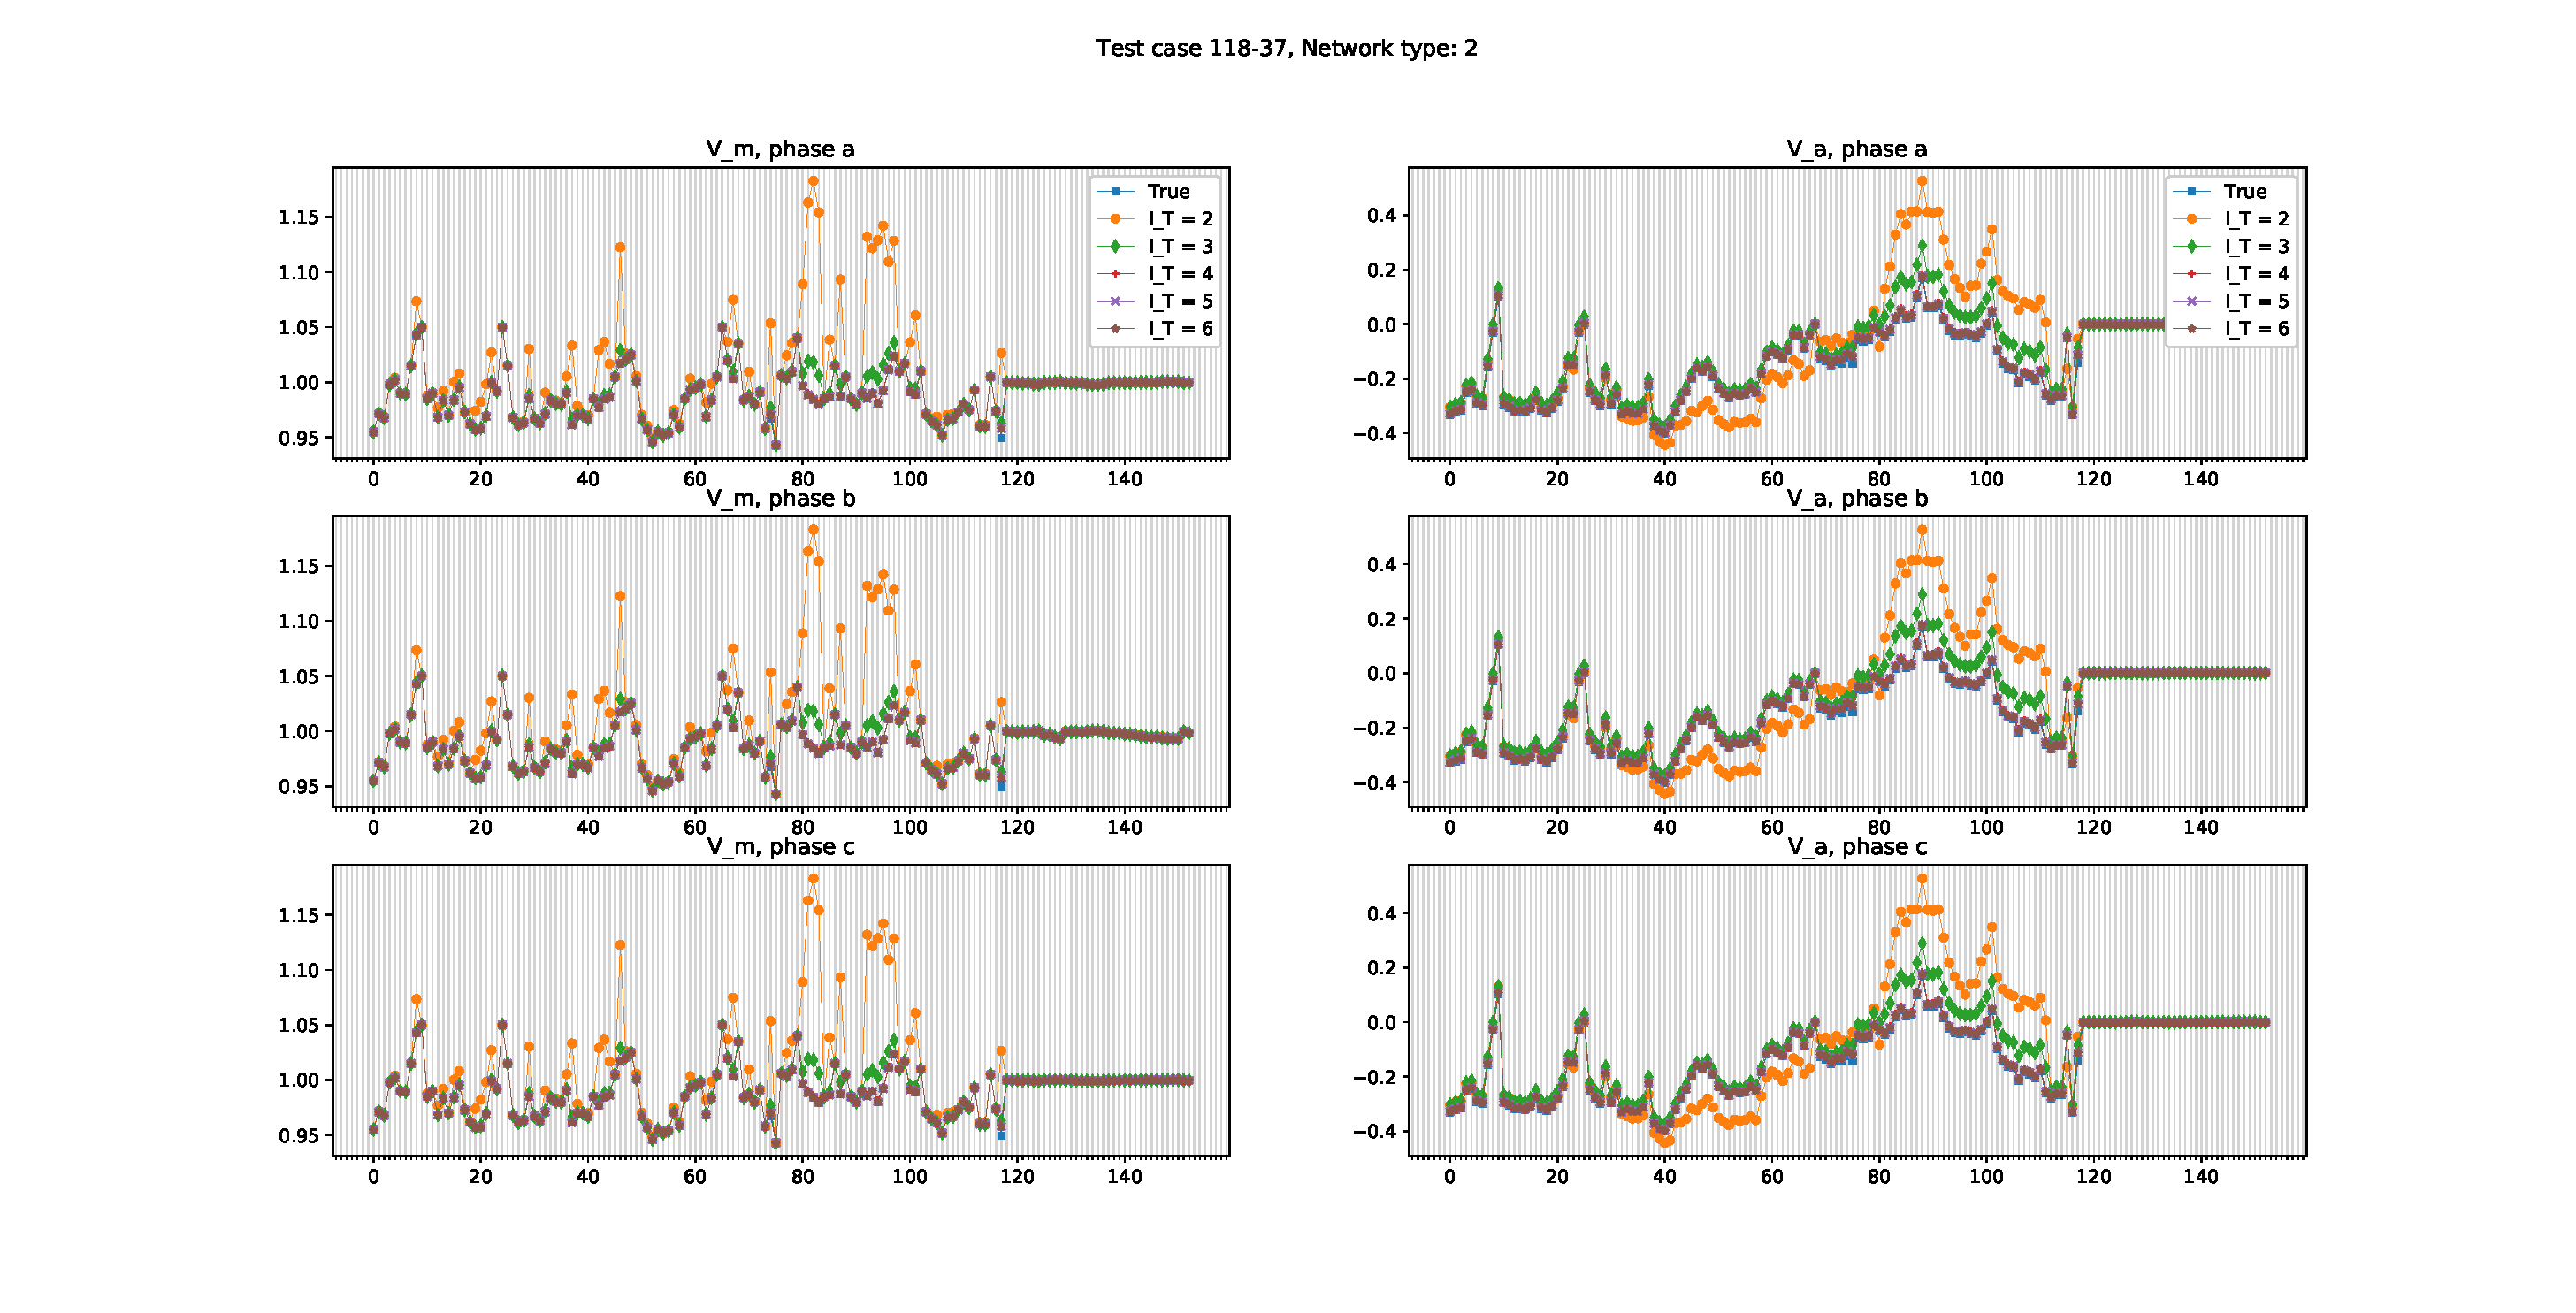
\includegraphics[width=\textwidth]{Images/MAI_N2.eps}
\caption{Voltage profile (left: magnitude, right: angle) of the MAI-schemes with increasing number of subiterations, applied on homogeneous networks}\label{fig:MAIN2}
\end{figure}
\begin{figure}[h]
\centering
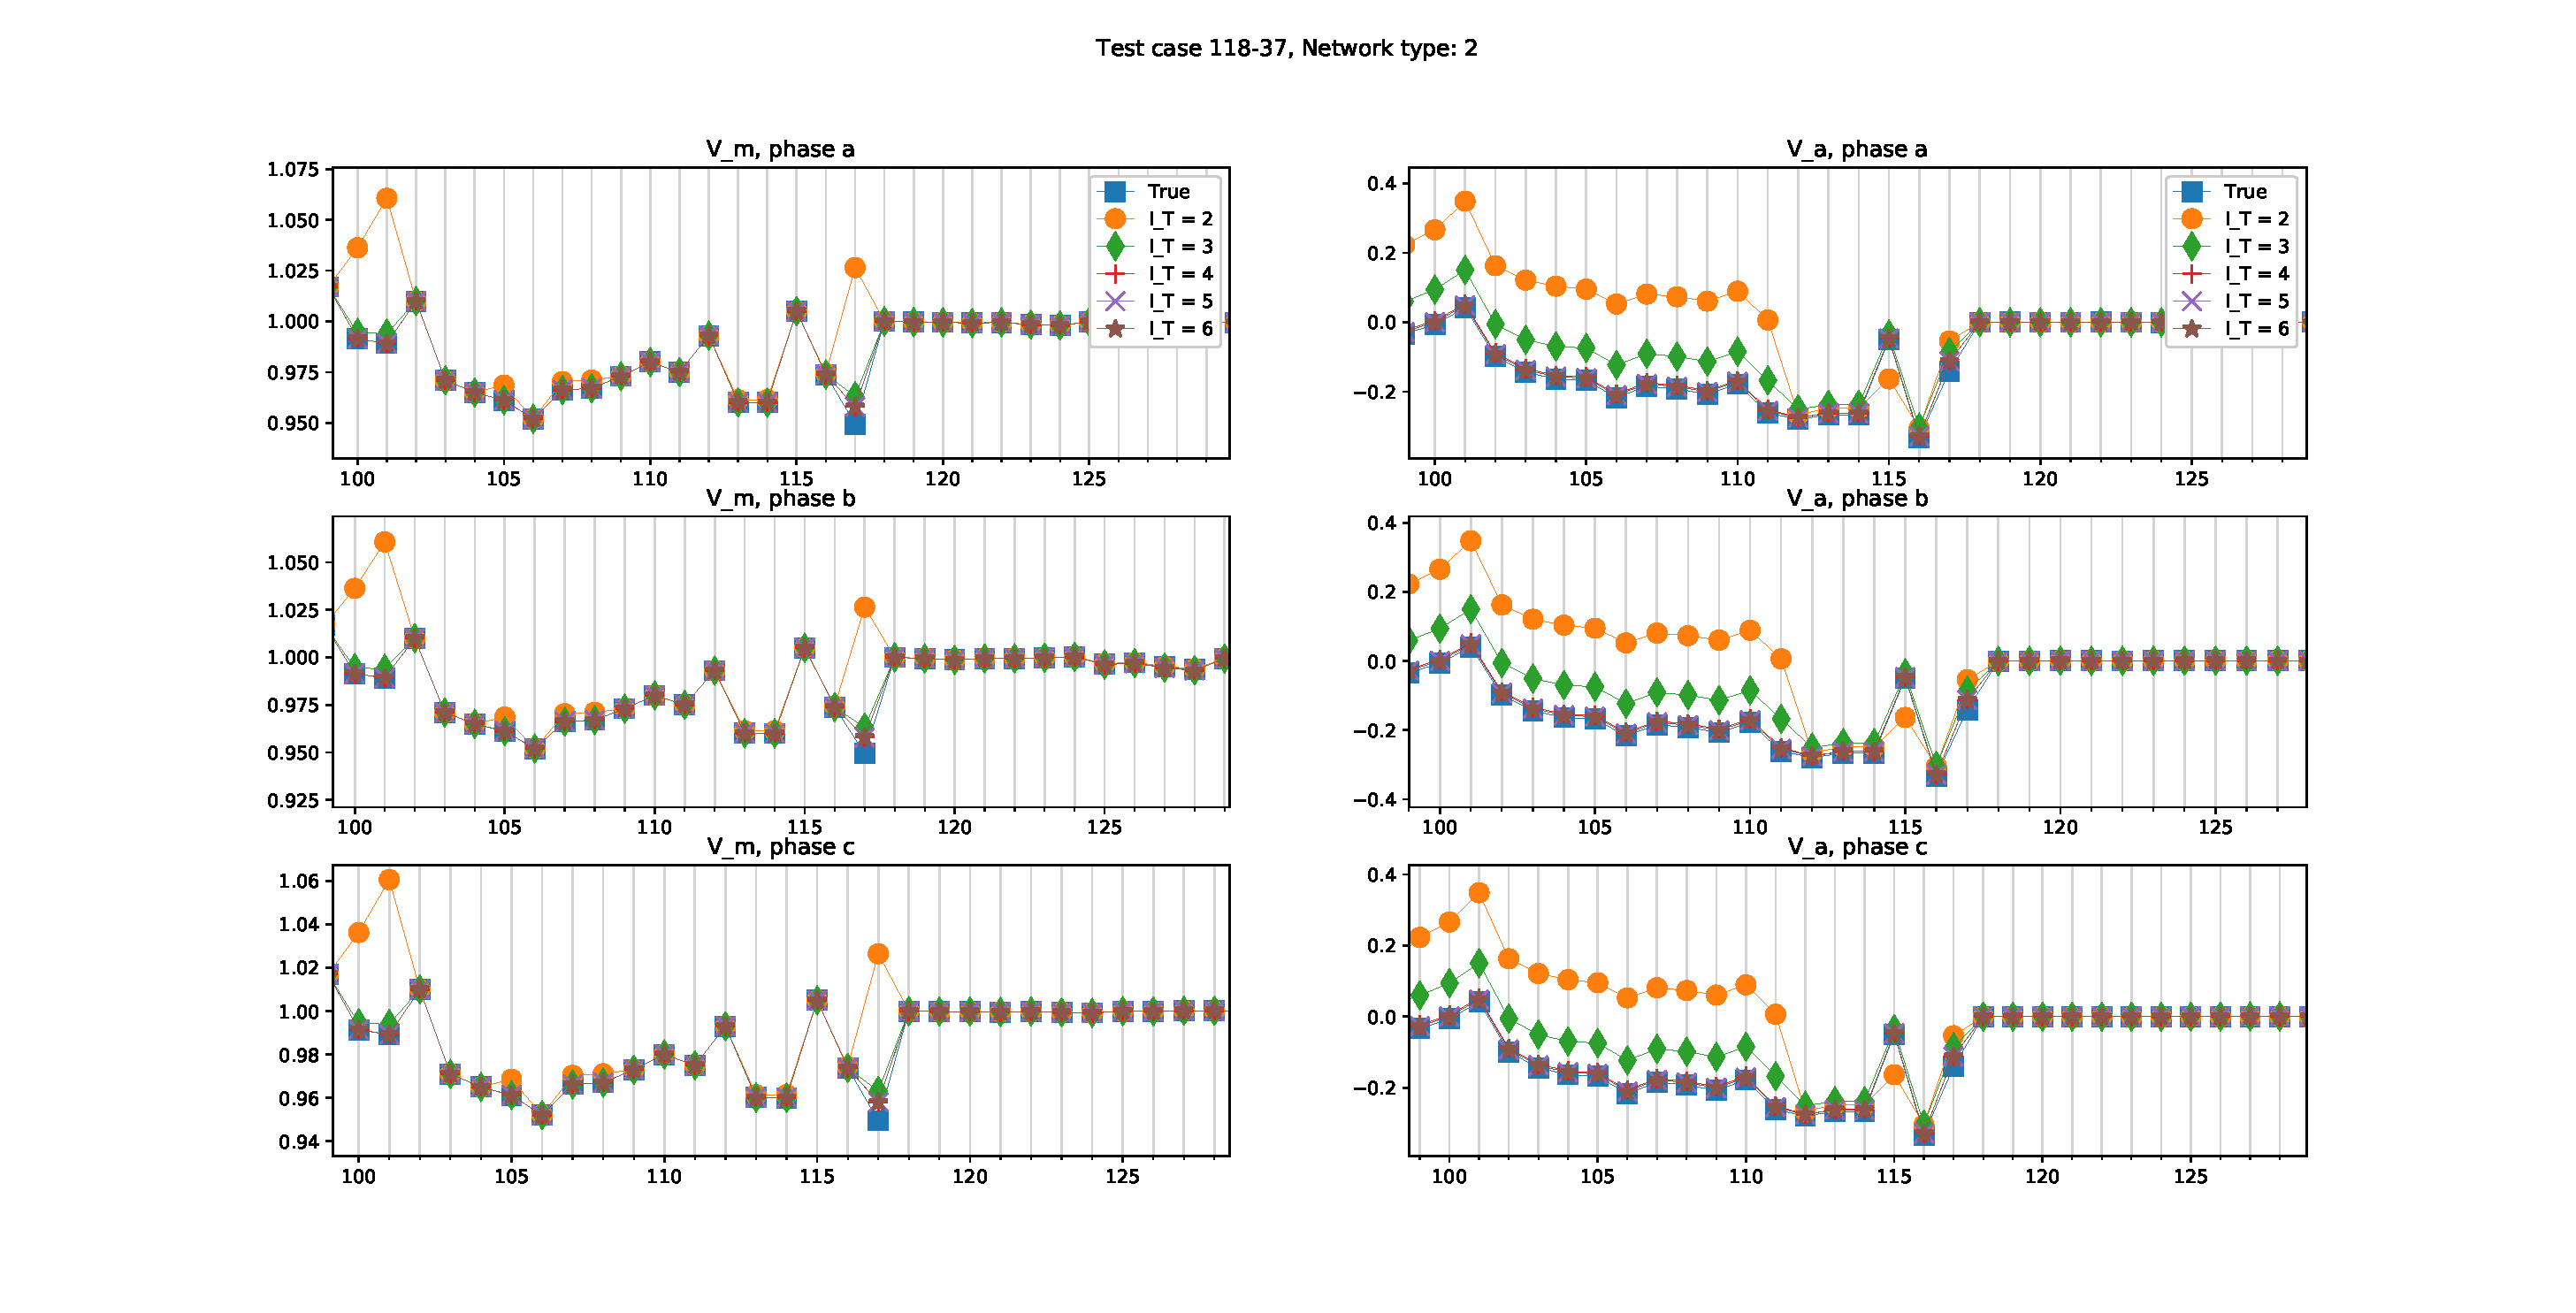
\includegraphics[width=\textwidth]{Images/Z_MAI_N2.eps}
\caption{A magnified version of figure \ref{fig:MAIN2} of the buses surrounding the connection bus.}\label{fig:ZMAIN2}
\end{figure}
\begin{figure}[h]
\centering
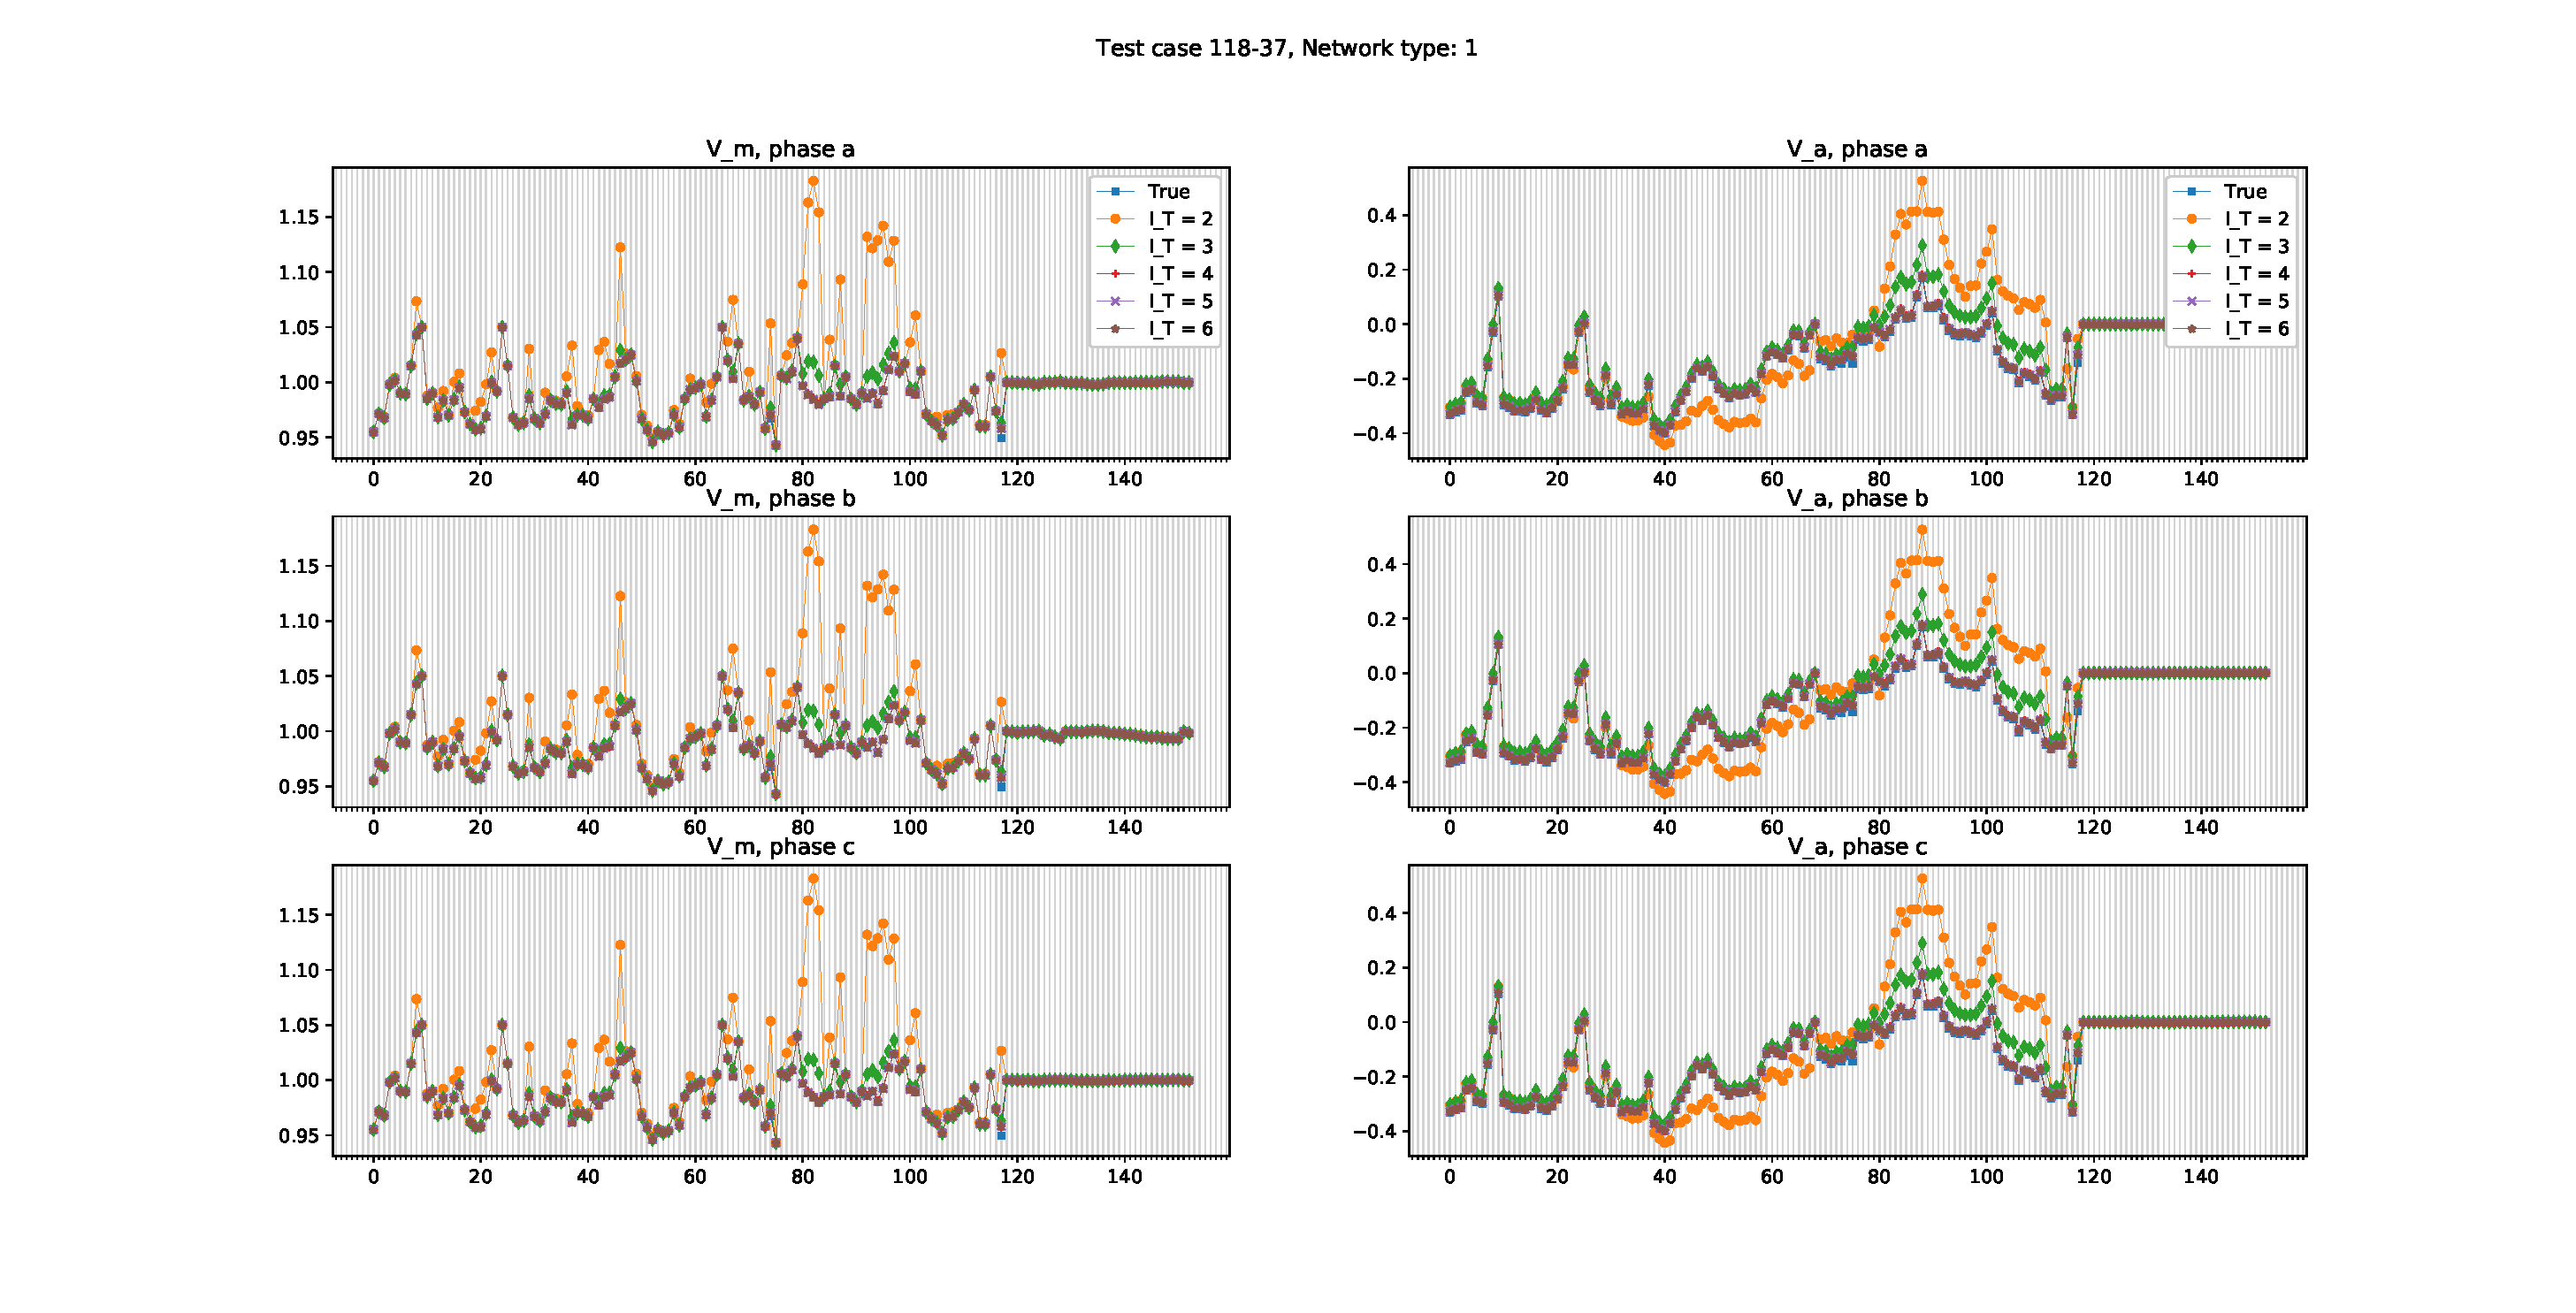
\includegraphics[width=\textwidth]{Images/MAI_N1.eps}
\caption{Voltage profile (left: magnitude, right: angle) of the MAI-schemes with increasing number of subiterations, applied on hybrid networks}\label{fig:MAIN1}
\end{figure}
\begin{figure}[h]
\centering
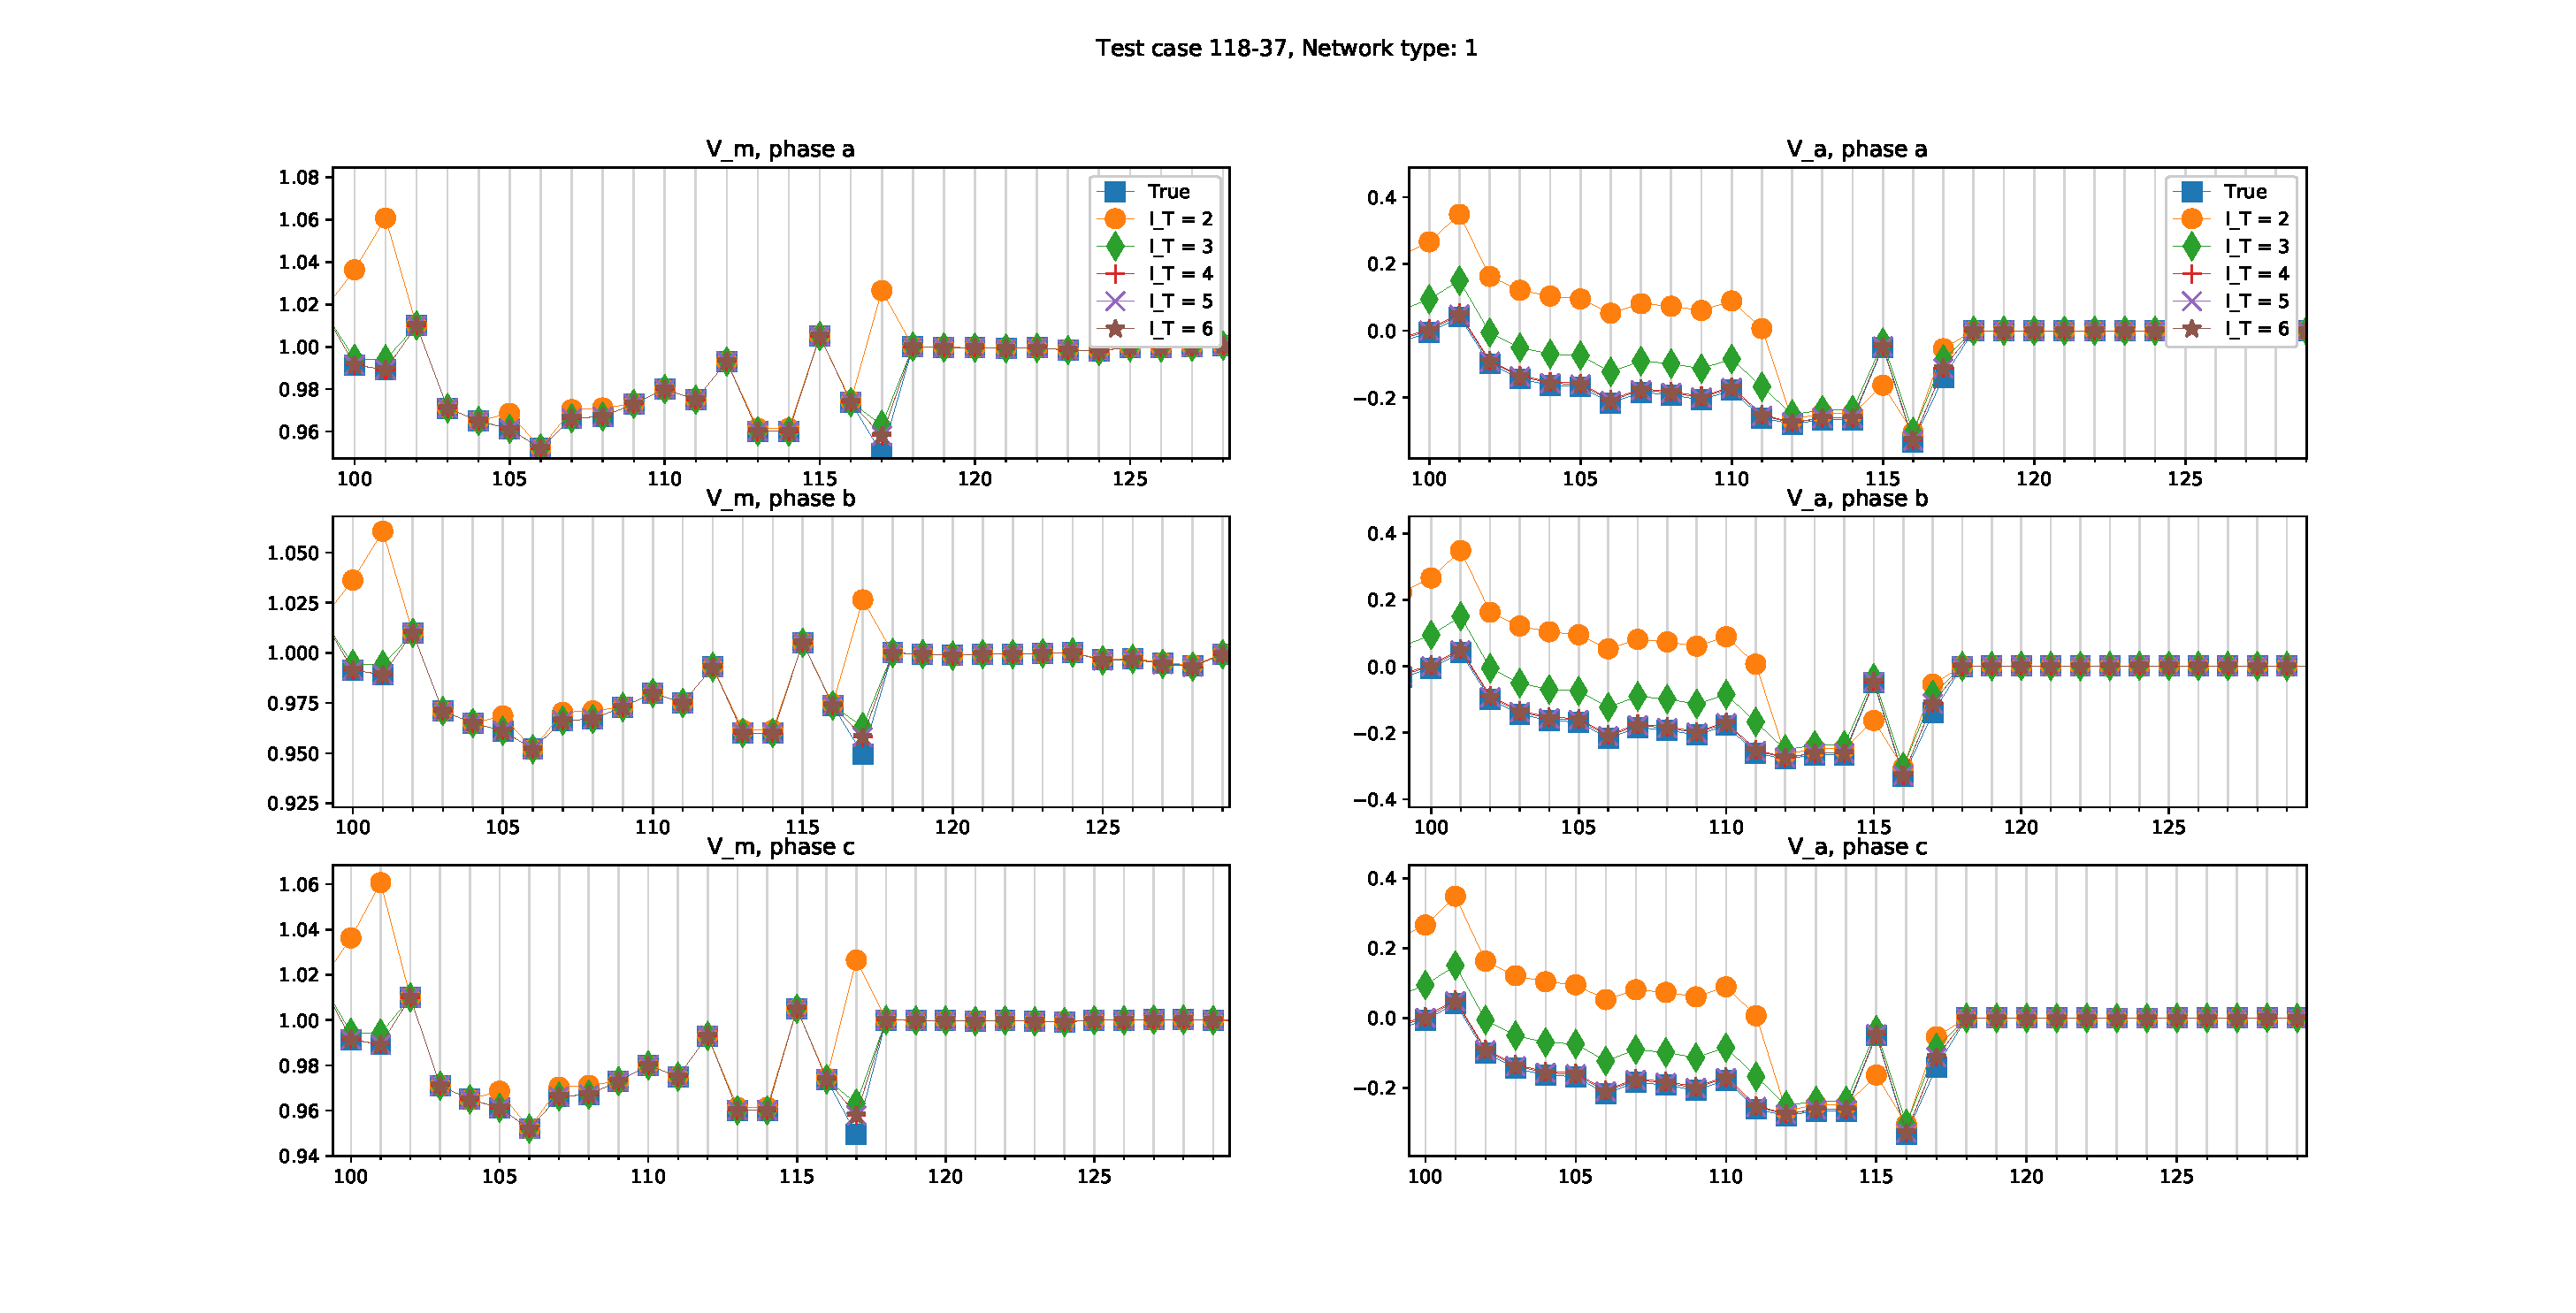
\includegraphics[width=\textwidth]{Images/Z_MAI_N1.eps}
\caption{A magnified version of figure \ref{fig:MAIN1} of the buses surrounding the connection bus.}\label{fig:ZMAIN1}
\end{figure}

\end{document}
